%% ============================================================================
%% Informe de Etapa 2: Diseño e Implementación Inicial. INFO1197, II-2026.
%% Nieves & Antivil. Proyecto LaTeX autocontenido, derivado del preámbulo de
%% thesis/draft/main.tex (memoir 12 pt, Palatino, biblatex-apa con biber; sin
%% amsmath; \mathrm{} y no \text{}; ancho de texto 382.6 pt).
%%
%% Construir desde PowerShell con MiKTeX:
%%   pdflatex -interaction=nonstopmode -output-directory=build main.tex
%%   biber --input-directory build --output-directory build main
%%   pdflatex -interaction=nonstopmode -output-directory=build main.tex   (dos veces)
%%   Copy-Item build/main.pdf main.pdf
%%
%% Las figuras F1-F4, F6-F7, A1-A2 y el cuadro T5 se leen directamente de ../figuras/*.pdf
%% (\graphicspath abajo), para que cada construcción tome la última versión.
%% La carpeta informe/figuras/ es una copia antigua y ya no se usa. Para
%% subir el proyecto a Overleaf hay que llevar también ../figuras/.
%% ============================================================================
\documentclass[12pt,oneside,spanish,oldfontcommands]{memoir}
\usepackage[utf8]{inputenc}
\usepackage[backend=biber,style=apa]{biblatex}
\addbibresource{referencias.bib}
\DeclareLanguageMapping{spanish}{spanish-apa}
\usepackage{mathpazo}
\usepackage[T1]{fontenc}
\setcounter{secnumdepth}{2}
\setcounter{tocdepth}{2}
\setlength{\parskip}{\smallskipamount} % la plantilla usa \medskipamount; reducido por el límite de treinta páginas
\setlength{\parindent}{0pt}
\setlength{\headheight}{16pt}
\usepackage{babel}
\usepackage{booktabs}
\usepackage{float}
\usepackage{placeins}
\usepackage{url}

\usepackage{endnotes}
\addto\shorthandsspanish{\spanishdeactivate{~<>.}}

\usepackage{array}
\usepackage{rotfloat}
\usepackage{textcomp}
%\usepackage{amssymb,amsmath}  % se mantiene comentado como en la plantilla; con amsmath memoir numera las ecuaciones como (N.0)
\usepackage{graphicx}
\graphicspath{{../figuras/}}
\usepackage{esint}
\usepackage{csquotes}
\usepackage{hyperref}
\usepackage{xurl}
\usepackage[none]{hyphenat}
\usepackage{longtable}
\newcolumntype{L}[1]{>{\raggedright\arraybackslash}p{#1}}
% nombres de archivo, módulos, rutas y opciones en cuadros; cortan solo en _ / - .
\DeclareUrlCommand\archivo{\urlstyle{tt}\def\UrlBreaks{\do\_\do\/\do\-\do\.}\def\UrlBigBreaks{}}

\usepackage{dsfont}
\usepackage{algorithm}
\usepackage{multirow}
\usepackage{algorithmicx}
\usepackage{algpseudocode}

\algdef{SE}[VARIABLES]{Variables}{EndVariables}
   {\algorithmicvariables}
   {\algorithmicend\ \algorithmicvariables}
\algnewcommand{\algorithmicvariables}{\textbf{global variables}}
\floatname{algorithm}{Algoritmo}
\algrenewcommand\algorithmicrequire{\textbf{Entrada:}}
\algrenewcommand\algorithmicensure{\textbf{Salida:}}
\algrenewcommand\algorithmicreturn{\textbf{devolver}}
\algrenewcommand\algorithmicfor{\textbf{para}}
\algrenewcommand\algorithmicforall{\textbf{para todo}}
\algrenewcommand\algorithmicdo{\textbf{hacer}}
\algrenewcommand\algorithmicend{\textbf{fin}}
\algrenewcommand\algorithmicif{\textbf{si}}
\algrenewcommand\algorithmicthen{\textbf{entonces}}
\algrenewcommand\algorithmicelse{\textbf{si no}}
\algrenewcommand\algorithmicwhile{\textbf{mientras}}
\addto\captionsspanish{\renewcommand{\appendixname}{Anexo}}

\newcommand{\Tau}{\mathrm{T}}
\newcommand{\I}{\mathds{1}}

\makeatletter
\@ifundefined{showcaptionsetup}{}{%
 \PassOptionsToPackage{caption=false}{subfig}}
\usepackage{subfig}
\renewcommand{\ALG@name}{Algoritmo}
\makeatother

%% Pies de figura y de cuadro en tamaño pequeño: el bloque de texto mide 548,5 pt
%% de alto y las vistas, hasta 536 pt; cada vista lleva su clave de notación
%% impresa al pie de la propia figura, por lo que el pie LaTeX solo da el mensaje.
\captionnamefont{\footnotesize\bfseries}
\captiontitlefont{\footnotesize}
%% Encabezados de capítulo compactos (el estilo de la plantilla deja un tercio de
%% página en blanco por capítulo; el informe tiene límite de treinta páginas).
\setlength{\beforechapskip}{0pt}
\setlength{\midchapskip}{4pt}
\setlength{\afterchapskip}{12pt}
\renewcommand{\chapnamefont}{\normalfont\large\bfseries}
\renewcommand{\chapnumfont}{\normalfont\large\bfseries}
\renewcommand{\chaptitlefont}{\normalfont\LARGE\bfseries\raggedright}
\setlength{\cfttablenumwidth}{3.2em}
\cftsetindents{section}{1.5em}{2.7em}
\cftsetindents{subsection}{4.2em}{3.2em}
%% Flotantes: las vistas miden hasta 19 cm de alto; sin estos valores un flotante
%% más alto que \topfraction y más bajo que \floatpagefraction queda varado.
%% Espacios verticales compactos alrededor de títulos de sección, flotantes y cuadros
%% largos, por el mismo límite de páginas.
\setbeforesecskip{-2.6ex plus -0.6ex minus -0.2ex}
\setaftersecskip{1.3ex plus 0.2ex}
\setbeforesubsecskip{-2.2ex plus -0.5ex minus -0.2ex}
\setaftersubsecskip{1.0ex plus 0.2ex}
\setlength{\textfloatsep}{12pt plus 2pt minus 4pt}
\setlength{\floatsep}{10pt plus 2pt minus 2pt}
\setlength{\intextsep}{10pt plus 2pt minus 2pt}
\setlength{\LTpre}{6pt}
\setlength{\LTpost}{6pt}
\renewcommand{\topfraction}{0.95}
\renewcommand{\bottomfraction}{0.6}
\renewcommand{\textfraction}{0.05}
\renewcommand{\floatpagefraction}{0.8}

%% Evidencia: enlaces verificados o archivos incluidos en el paquete local.

\begin{document}

\sloppy

\vspace*{-6\baselineskip}
\pagenumbering{gobble}
\hspace*{-0.0\textwidth}
\includegraphics[width=\textwidth]{images/Logo_depto_ing_informatica.png}

\vspace{2.5cm}

\begin{center}
    {\large\textbf{INFORME DE ETAPA 2:\\ DISEÑO E IMPLEMENTACIÓN INICIAL}}
\end{center}

\vspace{1.5cm}

\begin{center}
Trabajo de Título\\[0.6em]
\textbf{IMPLEMENTACIÓN VERIFICADA EN C++ DE DW-NOMINATE PARA EL ESTUDIO
DEL CAMBIO IDEOLÓGICO EN LA CÁMARA DE DIPUTADOS DE CHILE}
\end{center}

\vspace{2.5cm}

\begin{center}
por
\par\end{center}

\begin{center}
PABLO ANTIVIL MORALES \& ROBERTO NIEVES TOCORNAL\vspace{1.5cm}
\par\end{center}

\begin{center}
Informe de etapa del curso INFO1197 Trabajo de Título\\
Facultad de Ingeniería, Universidad Católica de Temuco
\par\end{center}

\begin{center}
Profesor guía: Dr. Julio Rojas Mora
\par\end{center}

\begin{center}
- Temuco, 9 de octubre de 2026 -
\par\end{center}

\clearpage

\pagenumbering{roman}

\tableofcontents{}

\clearpage

\listoffigures
\clearpage

\listoftables

\clearpage

\pagenumbering{arabic}
\setcounter{page}{1}

\setlength{\tabcolsep}{4pt}
%% Cuerpo continuo: cada capítulo sigue en la misma página tras vaciar los
%% flotantes pendientes, por el límite de treinta páginas de cuerpo. La
%% bibliografía y los anexos vuelven a empezar en página nueva.
\renewcommand{\clearforchapter}{\par\FloatBarrier\vspace{2\baselineskip}}
\chapter{Introducción}
\label{cap:introduccion}

\section{Propósito y forma del informe}
\label{sec:proposito}

Este informe es el entregable de la Etapa 2, Diseño e Implementación Inicial, del curso
INFO1197 Trabajo de Título. Según lo acordado con el profesor guía el 5 de octubre de 2026,
cada etapa se entrega como un informe propio, organizado por los criterios de su pauta, con el
detalle en anexos y la evidencia enlazada al repositorio. Los capítulos \ref{cap:retro} a
\ref{cap:documentacion} siguen, en orden y con su título, los cuatro criterios de la Etapa 2
(20, 10, 55 y 15\,\%). Los enlaces remiten a destinos comprobados o archivos incluidos en el paquete local;
el anexo \ref{anexo:procedencia} distingue publicación, revisión local y acciones de entrega.

El trabajo reimplementa y refactoriza en C++ un instrumento científico heredado, el programa
DW-NOMINATE escrito en Fortran \parencite{poole2005spatial}, por mantenibilidad, operabilidad y
rendimiento. Ninguna de esas ventajas se da por demostrada: aquí son criterios de diseño, y se
miden en las etapas 3 y 4. La sustitución de las búsquedas heredadas por optimizadores modernos
es una intervención deliberada, aislada en un segundo motor. El caso chileno ejercita el
instrumento en condiciones operativas reales, y los datos de VoteView
\parencite{boche2018voteview} aportan una comparación adicional de confianza.

\section{Problema, objetivos y requisitos}
\label{sec:recap}

El planteamiento completo, con las partes interesadas, los criterios SMART y la evaluación de
alternativas, está en el Informe de Etapa 1 (\href{run:../evidence/informe-etapa-1.pdf}{Informe de Etapa 1}).

\paragraph{Problema.} La plataforma QueVotan estima las posiciones ideológicas de los
diputados con un mapa independiente por periodo, y dos mapas independientes no comparten
origen, orientación ni escala \parencite{herron2004scale}: el desplazamiento entre periodos no
es observable. DW-NOMINATE \parencite{poole2005spatial} estima todos los periodos en un marco
común, pero su implementación canónica es un programa Fortran de 2004, monohilo y no pensado
para ser auditado. Falta una implementación abierta, mantenible y auditable, y una
reimplementación no vale mientras no se establezca con qué fidelidad reproduce a la
referencia; la coincidencia de las salidas finales no basta, porque un defecto de indexación
abrió una distancia grande en log-verosimilitud con la primera dimensión prácticamente igual
\parencite{nieves2026jcc}.

\paragraph{Objetivos.} El objetivo general es desarrollar una implementación verificada en
C++ del modelo DW-NOMINATE que permita estimar posiciones ideológicas comparables en el
tiempo para la Cámara de Diputados de Chile. Los específicos son los de la Etapa 1, con los
plazos ajustados de la sección \ref{sec:cambios-e1}; la sección \ref{sec:propuesta-chile}
propone reformular OE3.
\begin{itemize}
  \item \textbf{OE1.} Implementar en C++ dos motores DW-NOMINATE, uno fiel al programa de
  referencia de 2004 y otro con optimizador moderno, con paridad de entradas y salidas
  respecto de la referencia.
  \item \textbf{OE2.} Verificar la fidelidad de la implementación frente a la referencia
  canónica sobre paneles estadounidenses y chilenos, midiendo la sensibilidad de la segunda
  dimensión al modelo temporal, al marco de coordenadas y a los valores iniciales.
  \item \textbf{OE3.} Estimar el desplazamiento de los partidos en la primera dimensión
  durante el 55.º periodo legislativo (2018--2022) con inferencia por bootstrap paramétrico,
  como caso de validación del instrumento.
\end{itemize}

\paragraph{Requisitos.} Se derivaron del artefacto construido, según lo establecido con el
propietario el 3 de septiembre de 2026 (cuadro \ref{tab:requisitos}); RNF09 se agregó después
de la Etapa 1. Las secciones \ref{sec:atributos} y \ref{sec:trazabilidad} los trazan al
diseño.

\begin{table}[htbp]
\centering
\caption{Requisitos funcionales y no funcionales del Informe de Etapa 1, con RNF09.}
\label{tab:requisitos}
\footnotesize
\begin{tabular}{L{1.1cm}L{4.9cm}L{1.1cm}L{5.0cm}}
\toprule
ID & Requisito funcional & ID & Requisito no funcional \\
\midrule
RF01 & Ingesta y validación de entradas & RNF01 & Fidelidad, dentro de una tolerancia
declarada por panel \\
RF02 & Valores iniciales declarados y reproducibles & RNF02 & Determinismo con cualquier
número de hilos \\
RF03 & Estimación estática & RNF03 & Reproducibilidad desde un clon limpio \\
RF04 & Estimación dinámica & RNF04 & Rendimiento, medido a un hilo sin alterar resultados \\
RF05 & Motor fiel & RNF05 & Portabilidad, Windows y Linux \\
RF06 & Motor moderno & RNF06 & Trazabilidad numérica \\
RF07 & Exportación en el marco del optimizador & RNF07 & Publicación \\
RF08 & Verificación en tres niveles & RNF08 & Control de versiones \\
RF09 & Informe de comparación & RNF09 & Mantenibilidad y auditabilidad \\
RF10 & Bootstrap paramétrico & & \\
RF11 & Inferencia sobre medianas de partido & & \\
RF12 & Sensibilidad al diseño & & \\
\bottomrule
\end{tabular}
\end{table}

\section{Los cuatro referentes}
\label{sec:referentes}

El informe distingue cuatro variantes del instrumento (cuadro \ref{tab:referentes}); el
original de 2004 y wmay nunca se tratan como un único «Fortran».

\begin{table}[htbp]
\centering
\caption{Los cuatro referentes que el informe nombra.}
\label{tab:referentes}
\footnotesize
\begin{tabular}{L{3.9cm}L{5.6cm}L{2.8cm}}
\toprule
Variante & Qué es & Rol en este trabajo \\
\midrule
Original 2004 (\archivo{DW-NOMINATE-2004.FOR}) & distribución de Poole y Rosenthal
\parencite{poole2005spatial}; SVD de IMSL; salvaguarda GRID & referencia histórica \\
wmay (\archivo{DW-NOMINATE-wmay.f}) & adaptación \parencite{wmay_dwnominate} con
\texttt{DGESDD} de LAPACK, sin GRID, acoplada a R & reproducción y evaluador común \\
Fiel C++ & traducción de las rutinas, corregida y configurada para compararse con wmay &
instrumento reimplementado \\
Moderno C++ & el mismo modelo con búsquedas de NLopt \parencite{johnson_nlopt} &
intervención \\
\bottomrule
\end{tabular}
\end{table}

\chapter{Incorpora la retroalimentación}
\label{cap:retro}

\section{Estado de la retroalimentación de la Etapa 1}
\label{sec:estado-retro}

El Informe de Etapa 1 se entregó el 4 de septiembre de 2026 (\href{run:../evidence/informe-etapa-1.pdf}{Informe de Etapa 1 entregado}). La revisión escrita anunciada no llegó como
documento; en la reunión del 5 de octubre el profesor guía informó que la Etapa 1 fue
calificada con 7,0 y que no quedaba retroalimentación pendiente. La única observación abierta
concierne a la implementación: el motor fiel debe alcanzar el rendimiento a un núcleo del
original 2004, revisando sus estructuras de datos (protocolos de la sección
\ref{sec:protocolos}). Su diseño está en la sección
\ref{sec:rendimiento} y en el registro RD-9; la implementación y la medición antes y después
corresponden a la Etapa 3, cuya pauta las pide.

\section{Indicaciones del profesor guía y cambios hechos}
\label{sec:indicaciones}

El cuadro \ref{tab:indicaciones} registra cada indicación del profesor guía desde el inicio
del curso, el cambio que produjo y dónde se ve.

\footnotesize
\begin{longtable}{L{1.6cm}L{3.4cm}L{4.8cm}L{2.4cm}}
\caption{Indicaciones del profesor guía, cambio hecho y dónde se ve.}\label{tab:indicaciones}\\
\toprule
Fecha y medio & Indicación & Cambio hecho & Dónde se ve \\
\midrule
\endfirsthead
\multicolumn{4}{l}{\footnotesize\emph{Cuadro \ref{tab:indicaciones}, continuación}}\\
\toprule
Fecha y medio & Indicación & Cambio hecho & Dónde se ve \\
\midrule
\endhead
\bottomrule
\endfoot
24 ago., mensaje del curso & Límite de treinta páginas; estructura de Cardiff; SWEBOK v4 como
guía de estándares & el cuerpo lleva lo que la pauta evalúa y el detalle va a anexos; cada
vista y decisión cita SWEBOK v4.0a, ISO/IEC/IEEE 42010, IEEE 1016 o UML 2.5.1 & todo el
informe \\
\addlinespace
3 sept., reunión & Derivar los requisitos de lo construido; el umbral RNF01 es del
propietario; no afirmar convergencia & cada decisión cita código o configuración con archivo y
línea; el valor del umbral queda abierto; ciclos fijos, sin prueba de convergencia & cuadro
\ref{tab:decisiones}; sección \ref{sec:experimental}; RD-5 \\
\addlinespace
28 sept., reunión semanal & Mejorar el rendimiento del motor fiel revisando punteros y
estructuras de datos & RNF04 precisado; OE1 con criterio medible y plazos; diseño de la mejora
(D-20, D-21) & sección \ref{sec:rendimiento}; RD-9 \\
\addlinespace
5 oct., reunión & Informe propio por etapa y criterio; diagramas según estándares; decisiones
con su porqué; rendimiento a un núcleo del Fortran & este informe; seis figuras de cuerpo, un cuadro de mecanismos y dos
figuras de anexo con notación declarada; decisiones con alternativa, razón y evidencia; nueve
registros & secciones \ref{sec:decisiones} y \ref{sec:registros} \\
\end{longtable}
\normalsize

\section{Cambios al contenido de la Etapa 1}
\label{sec:cambios-e1}

El Informe de Etapa 1 queda como se entregó. En el documento de trabajo de título
(\href{run:../evidence/documento-tesis-2026-10-04.pdf}{documento de tesis, 4 de octubre de 2026}) su contenido recibió
después cambios que no responden a una observación sobre la Etapa 1, sino a indicaciones
posteriores, a la auditoría de cada cifra contra su fuente y a una revisión adversarial
independiente: el capítulo 2 se completó, porque sus ecuaciones no coincidían con el código; se
agregó RNF09, Mantenibilidad y auditabilidad, que el propietario pide desde el 15 de abril de
2026 y que el diseño no tenía respaldado (cuadro \ref{tab:atributos}); el hito de octubre de
OE1 se acotó y la mejora completa medida pasó a inicios de diciembre, porque no cabe en cuatro
semanas junto con las pruebas de la Etapa 3 (RD-9); se retiraron o corrigieron cifras de los
capítulos 1 y 3, entre ellas la causa del caso de 61 de 168 legisladores; y el registro de
tareas salió del documento hacia la planilla y el repositorio (capítulo \ref{cap:avance}).

\section{Propuesta: el caso chileno como validación en condiciones operativas reales}
\label{sec:propuesta-chile}

Esta propuesta de los autores deriva de la reunión del 5 de octubre y queda pendiente de
confirmación en la revisión del 9 de octubre. En esa reunión el profesor guía describió el
trabajo como dos tareas, mostrar que el programa Fortran se puede replicar y que se puede
mejorar, con una validación cuantitativa contra el Fortran. OE3 enuncia el estudio chileno
«como caso de validación del instrumento», pero lo mantiene como objetivo propio. Se propone
que sea la validación en condiciones operativas reales que pide la pauta de la Etapa 4: si se
confirma, OE3 se reformula o se retira, RF10 a RF12 se trazan a esa validación y la tarea H1
queda resuelta en dos tareas, replicar y mejorar. Mientras no se confirme, los objetivos de la
sección \ref{sec:recap} siguen vigentes.

\section{Decisiones que quedan en manos del profesor guía}
\label{sec:decisiones-guia}

\begin{enumerate}
  \item Confirmación de la propuesta anterior y, con ella, de la descomposición de objetivos
  (tarea H1).
  \item Valor del umbral de fidelidad RNF01, criterio de aceptación de las pruebas
  exhaustivas (tareas C6 y H2); la sección \ref{sec:experimental} propone su forma.
  \item Ratificación del diseño principal de periodización del estudio chileno (D-16).
\end{enumerate}

El 5 de octubre se acordó entregar un informe propio como enlace. El límite de treinta
páginas se aplica por informe y al cuerpo como supuesto de trabajo, no como acuerdo ratificado.

\chapter{Avanza adecuadamente en el diseño}
\label{cap:avance}

\section{El backlog y su registro}
\label{sec:backlog}

El backlog se estableció en el Informe de Etapa 1, con veinticinco ítems en siete épicas, y
se amplió el 4 de septiembre de 2026 con nueve tareas de proceso (H1 a H9), pendientes de
adopción. Su definición está en el repositorio (\href{run:../evidence/research/backlog/README.md}{backlog}) y su
ejecución en la planilla compartida con el profesor guía (\href{https://docs.google.com/spreadsheets/d/1FXSB_2WqGL2TbOgw698gQEBTbL3nV7qXFypcflpYgEw/edit?gid=313395138}{planilla}).
Cada ítem lleva la categoría con que la pauta mide el avance. Dos cambios de
planificación del 4 de septiembre se declaran: E3 pasó de la Etapa 4 a la 2, porque es una
decisión de diseño con su insumo (D1) terminado, y H8 pasó de la Etapa 3 a la 2, porque es el
diseño experimental que G2 compromete. El cuadro \ref{tab:backlog} da el estado al 8 de
octubre de 2026. Planilla y backlog enlazados conservan estados anteriores: G2 y E3 sin empezar,
H8 pendiente y fecha antigua. Su sincronización sigue abierta (anexo
\ref{anexo:procedencia}).

{\scriptsize
\setlength{\tabcolsep}{3pt}
\begin{longtable}{L{0.55cm}L{6.8cm}L{1.45cm}L{1.2cm}L{2.2cm}}
\caption[Registro del backlog entero al 8 de octubre de 2026.]{Registro del backlog entero,
con el estado al 8 de octubre de 2026; en negrita, las tareas de diseño. Categorías: impl.,
implementación; doc., documentación; pub., publicación.}\label{tab:backlog}\\
\toprule
ID & Tarea & Categoría & Etapa & Estado \\
\midrule
\endfirsthead
\multicolumn{5}{l}{\scriptsize\emph{Cuadro \ref{tab:backlog}, continuación}}\\
\toprule
ID & Tarea & Categoría & Etapa & Estado \\
\midrule
\endhead
\bottomrule
\endfoot
A1 & Estimar posiciones en un panel de un periodo & impl. & E1 & listo \\
A2 & Trayectorias multiperiodo en un marco común & impl. & E1 & listo \\
A3 & Valores iniciales declarados y reproducibles & impl. & E1 & listo \\
A4 & Validar entrada y reportar faltas de semilla & impl. & E2 & sin empezar \\
A5 & Reconciliar marco de exportación y optimizador & impl. & E2 & sin empezar \\
B1 & Cuatro búsquedas por optimizadores modernos & impl. & E1 & listo \\
B2 & Evidencia controlada a ajustes igualados & prueba & E3 & sin empezar \\
C1 & Comparar cada rutina con el estado intermedio & prueba & E1 & listo \\
C2 & Puntuar el estado terminal con la referencia & prueba & E1 & listo \\
C3 & Comparar mapas con amplitud y reflexiones & prueba & E1 & listo \\
C4 & Regenerar el brazo dinámico estadounidense & prueba & E3 & sin empezar \\
C5 & Repetir la verificación en otra máquina & prueba & E3 & sin empezar \\
C6 & Acordar el umbral de fidelidad por panel & decisión & E2 & del propietario \\
D1 & Sensibilidad a periodo, semilla y compilación & prueba & E1 & listo \\
D2 & Registro de sensibilidad y su razón & doc. & E4 & sin empezar \\
E1 & Intervalos para las medianas de partido & impl. & E1 & listo \\
E2 & Elegibilidad, multiplicidad y robustez & impl. & E1 & listo \\
\textbf{E3} & \textbf{Diseño de periodización y discretización} & diseño & E2 & por ratificar \\
E4 & El caso como validación del instrumento & doc. & E4 & sin empezar \\
F1 & Compilar y ejecutar desde un clon limpio & pub. & E4 & sin empezar \\
F2 & Publicar el repositorio con licencia & pub. & E4 & sin empezar \\
G1 & Capítulos 1 a 3 y anexo de backlog & doc. & E1 & listo \\
\textbf{G2} & \textbf{Capítulo de diseño y diseño experimental} & diseño & E2 & hecho \\
G3 & Implementación y resultados preliminares & doc. & E3 & sin empezar \\
G4 & Documento completo y conclusiones & doc. & E4 & sin empezar \\
H1 & Descomposición de objetivos & decisión & E2 & propuesta \\
H2 & Acordar RNF01 antes de diseñar pruebas & decisión & E2 & del propietario \\
H3 & Puerta de paridad de entradas & impl. & E3 & por adoptar \\
H4 & Suite de pruebas como artefacto & impl. & E3 & por adoptar \\
H5 & Registro de números en la tesis & doc. & E3, E4 & por adoptar \\
H6 & Tabla de retroalimentación por etapa & doc. & E2 a E4 & hecho en E2 \\
H7 & Presupuesto de páginas & decisión & E2 & supuesto \\
\textbf{H8} & \textbf{Pruebas exhaustivas diseñadas antes de correr} & diseño & E2 & escrito; aprobar \\
H9 & Congelar dos días antes de cada etapa & proceso & E2 a E4 & al congelar \\
\end{longtable}
}

\section{Tareas de diseño frente al backlog entero}
\label{sec:tareas-diseno}

El registro base contiene treinta y cuatro ítems; siete propuestas I1--I7 de la Etapa 3
se agregaron localmente el 8 de octubre y se detallan en el anexo \ref{anexo:procedencia}.
Siguen pendientes de adopción, con responsables y horas propuestas. En el registro base, tres son de diseño (G2, E3, H8); los tres están
comprometidos en la Etapa 2 y tienen su artefacto escrito aquí (cuadro
\ref{tab:tareas-diseno}). Los tres diseños están disponibles; la ratificación de E3 y la
aprobación prevista en H8 siguen abiertas. No se confunde artefacto escrito con tarea aceptada. Los diez ítems de implementación se miden en las
etapas 3 y 4; seis están listos desde la Etapa 1.

\begin{table}[H]
\centering
\caption{Tareas de diseño de la Etapa 2: artefacto escrito y aceptación pendiente.}
\label{tab:tareas-diseno}
\footnotesize
\begin{tabular}{L{3.2cm}L{6.0cm}L{3.2cm}}
\toprule
Tarea & Artefacto & Estado \\
\midrule
G2, capítulo de diseño y diseño experimental & capítulo \ref{cap:diseno}: vistas, decisiones
con su razón, atributos de calidad, verificación por niveles, diseño experimental, mejora de
rendimiento, trazabilidad; anexos \ref{anexo:figuras} a \ref{anexo:rendimiento} & hecho \\
\addlinespace
H8, diseño de las pruebas exhaustivas & sección \ref{sec:experimental}; anexo
\ref{anexo:paneles} & escrito; aprobación y RNF01 del propietario \\
\addlinespace
E3, periodización y discretización & sección \ref{sec:algoritmos} y anexo \ref{anexo:chile}:
diseños de periodización y regla de discretización; D-16; RD-8 & escrito; ratificación pendiente \\
\bottomrule
\end{tabular}
\end{table}

I1--I6 añadirían seis ítems de implementación y llevarían la base de diez a dieciséis
solo después de su adopción; I7 es documentación. El cálculo $10/16$ daría 62,5\,\%; es
condicional: los seis ítems listos darían $6/16$ (37,5\,\%), y E3 exige ocho cierres.
La adopción revisará solapamientos con A4, A5 y H4. I6 conserva wmay como antecedente; se fija original
2004 como referente externo de la tesis (cuadro \ref{tab:protocolos}).

Las demás tareas de la Etapa 2 no son de diseño y su estado se declara sin atenuantes. A4 y
A5, de implementación en el motor fiel, no se iniciaron, porque en esta etapa no se
implementó código nuevo en los motores (sección \ref{sec:cambios}); su reprogramación se
decide con el profesor guía. C6 y H2 esperan la decisión del propietario; H1 tiene una
propuesta (sección \ref{sec:propuesta-chile}); H6 está hecha en el capítulo \ref{cap:retro};
H7 quedó resuelta como supuesto de trabajo, y H9 se ejecuta al congelar este informe.

\chapter[Diseña adecuadamente según estándares de calidad][Diseña según estándares de calidad]{Diseña adecuadamente según estándares de calidad}
\label{cap:diseno}

Este capítulo presenta el diseño del instrumento: estándares, seis figuras de cuerpo y un cuadro de mecanismos, las decisiones
que las explican con su razón y su evidencia, los atributos de calidad que persigue y el diseño
que las figuras no sustituyen. No presenta resultados: las cifras que lo evalúan pertenecen a
las etapas 3 y 4.

\section{Estándares y enfoque}
\label{sec:estandares}

El diseño se describe desde varios puntos de vista, cada uno dirigido a una preocupación de
las partes interesadas, como prescriben ISO/IEC/IEEE 42010 \parencite{iso42010}, IEEE 1016
\parencite{ieee1016} y SWEBOK \parencite[cap.~2, §2.1]{swebok2025}, con la separación en vistas
de \textcite{kruchten1995views}. Cada vista responde una pregunta, enunciada en el párrafo que
la introduce; su pie da el mensaje y la clave al pie de la figura define toda marca que no sea
UML. Las vistas usan UML 2.5.1 \parencite{omg_uml251} como notación estructural y de
comportamiento \parencite[cap.~11, §2]{swebok2025}: contexto (F1), casos de uso (F2), modelo conceptual
(F6), clases (A1), actividad (F4, F7) y secuencia (A2). F3 es una correspondencia de
responsabilidades y T5 un cuadro de mecanismos; ninguno pretende expresar dependencias UML. Cinco
principios gobiernan el sistema: una tubería por lotes sobre archivos \parencite[cap.~2,
§2.2]{swebok2025}; la separación de responsabilidades orientada al ocultamiento de información \parencite{parnas1972criteria} en el motor
fiel \parencite[cap.~3, §1.4]{swebok2025}; la concurrencia y el manejo de errores como
decisiones explícitas \parencite[cap.~3, §3.1 y §3.5]{swebok2025}; el motor moderno como
variante de una línea de productos \parencite[cap.~3, §3.8]{swebok2025}; y la verificación
como parte del sistema, con la referencia como oráculo \parencite[cap.~5, §1.2.7]{swebok2025}.
Cada decisión que explica una vista se cita como D-xx, con la numeración del registro de la
tesis (D-01 a D-21) continuada desde D-22, y se reúne con su razón y su evidencia en la sección
\ref{sec:decisiones}, como pide SWEBOK \parencite[cap.~3, §4.6]{swebok2025}. Cada elemento
dibujado tiene una cita de archivo y línea (\href{run:../figuras/FACTS.md}{juego de auditoría});
la notación está en el anexo \ref{anexo:figuras}.

\section{Vistas del instrumento y mecanismos numéricos}
\label{sec:vistas}

\subsection{Contexto y alcance del instrumento}
\label{sec:F1}

¿Quién usa el instrumento, con qué entradas y para obtener qué? En la figura \ref{fig:F1}, el
analista declara un panel, semillas y el motor, con lo que ejecuta una variante identificada
(cuadro \ref{tab:referentes}), y recibe coordenadas y parámetros; el verificador solicita
comparaciones. Son externos las fuentes de paneles (VoteView \parencite{boche2018voteview}; la
base de QueVotan y los datos de \textcite{fabrega2025ideological}), el servicio de semillas
\parencite{wnominate_pkg} y la referencia wmay, que devuelve coordenadas o una
log-verosimilitud. El portal en R es la entrada común a los dos motores y a la referencia,
cuyos binarios también pueden ejecutarse directamente; aplica el linaje del motor fiel y sella
cada corrida aceptada (D-24, D-30). La tubería es por lotes sobre archivos porque la referencia solo lee y escribe
archivos; la integración con QueVotan (anexo \ref{anexo:contratos}) es externa a este
trabajo.

\begin{figure}[tbp]
\centering
\makebox[\textwidth][c]{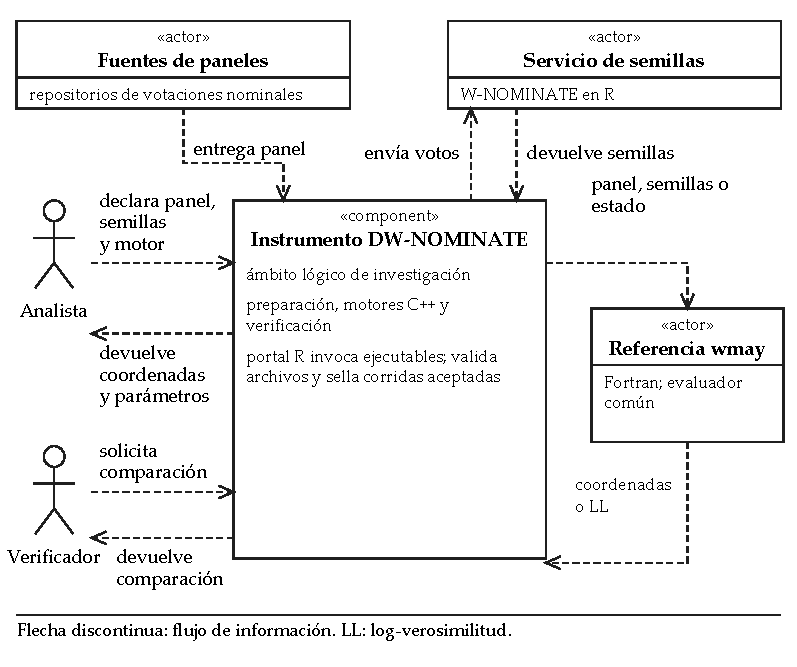
\includegraphics[width=13.5cm]{F1-contexto.pdf}}
\caption[F1. Contexto del instrumento]{Contexto lógico del instrumento de investigación. Ruta común: portal R, ejecutables y validación de archivos (D-24, D-30).}
\label{fig:F1}
\end{figure}

\subsection{Objetivos de los usuarios}
\label{sec:F2}

¿Qué puede hacer cada rol con el instrumento? En la figura \ref{fig:F2}, el analista declara
panel y semillas y estima posiciones, caso abstracto que se especializa en estático (RF03) y
dinámico (RF04), con el motor fiel o el moderno (RF05, RF06); la carga y validación de
entradas (RF01) ocurre dentro de la estimación. Validar con el caso chileno (RF10 a RF12) es
un flujo de investigación que reutiliza la estimación y no una función de la línea de
comandos. El sujeto incluye estimación, validación y comparación, y la elipse está dentro;
la reformulación del objetivo chileno sigue siendo propuesta de la sección
\ref{sec:propuesta-chile}. El verificador compara contra wmay (RF08, RF09); ambos roles pueden
ser la misma persona. Las narrativas de cada caso están en el anexo \ref{anexo:narrativas}.

\begin{figure}[tbp]
\centering
\makebox[\textwidth][c]{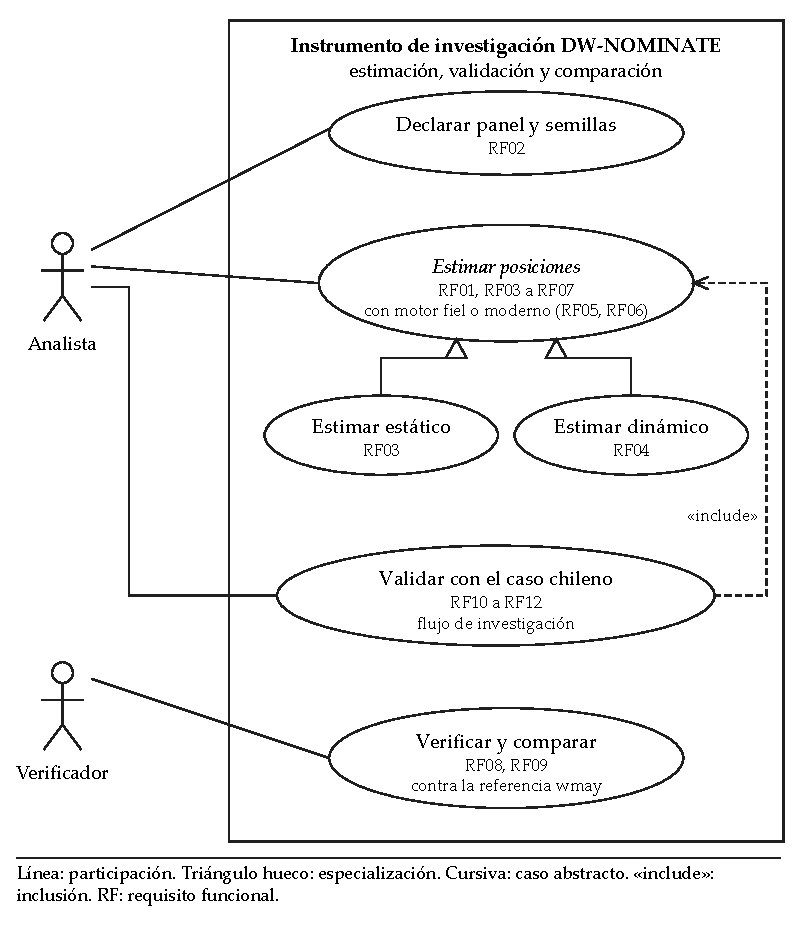
\includegraphics[width=13.5cm]{F2-casos-de-uso.pdf}}
\caption[F2. Objetivos de los usuarios]{Casos de uso del instrumento de investigación, que comprende estimación y validación. RF remite a los requisitos vigentes; la propuesta sobre Chile sigue pendiente.}
\label{fig:F2}
\end{figure}

\subsection{Del Fortran al C++: organización}
\label{sec:F3}

¿Dónde quedó cada responsabilidad del instrumento heredado? La figura \ref{fig:F3}
corresponde responsabilidades, sin superponer el grafo de dependencias. Distingue el programa
con archivos y estado \texttt{COMMON} de 2004 de la subrutina \texttt{dwnom} con módulos y
envoltorios de wmay. La derecha identifica entrada, configuración explícita, orquestación,
búsquedas, geometría, verosimilitud y soporte en el motor fiel. El catálogo de rutinas y el
grafo de inclusiones se documentan en el anexo \ref{anexo:correspondencia}.

El estado sigue concentrado en DWNominate para permitir el volcado por fases (D-22); las
búsquedas son funciones libres (D-23). \texttt{GRID} queda tras un interruptor (D-24) y el
perfil comparado usa \texttt{DGESDD} (D-01). Esa organización persigue mantenibilidad
\parencite{parnas1972criteria}; no demuestra ocultamiento completo ni una mejora medida.

\begin{figure}[tbp]
\centering
\makebox[\textwidth][c]{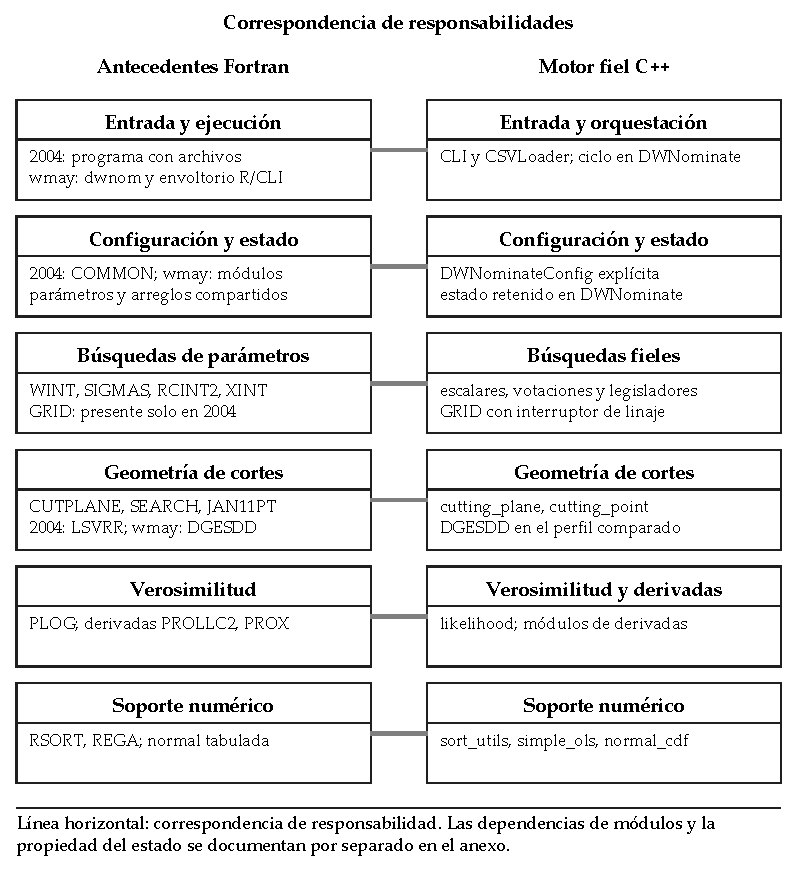
\includegraphics[width=13.5cm]{F3-fortran-a-cpp.pdf}}
\caption[F3. Correspondencia de responsabilidades]{Correspondencia de responsabilidades entre original 2004, wmay y fiel C++; catálogo de rutinas en el anexo \ref{anexo:correspondencia}.}
\label{fig:F3}
\end{figure}

\subsection{Ciclo de estimación compartido}
\label{sec:F4}

La figura \ref{fig:F4} ordena las actualizaciones de parámetros, votaciones y
legisladores, con evaluaciones intermedias. Tras cargar panel y semillas, la validez exige
un margen de minoría de al menos $2{,}5$\,\%. El corte usa \texttt{CUTPLANE} en 2D o
\texttt{JAN11PT} en 1D, seguido de \texttt{RCINT2}. El perfil wmay/fiel repite $T$ ciclos
fijos y exporta parámetros terminales (D-07); el resumen fiel mezcla fases (M-02, I2).
No hay prueba de convergencia. Compartir este flujo
no garantiza cifras iguales: la verosimilitud no es cóncava y se compara a ciclos igualados
(algoritmo \ref{alg:ciclo}; anexo \ref{anexo:perfil}).

\paragraph{Concurrencia.} El motor fiel usa OpenMP en votaciones, legisladores y la
verosimilitud de las búsquedas globales; la evaluación entre fases es serial; la referencia ejecuta todas las fases secuencialmente
\parencite[cap.~3, §3.1]{swebok2025}. Para conciliar paralelismo y determinismo (RNF02),
ninguna cantidad de punto flotante se reduce en una región paralela: la verosimilitud se
acumula por legislador y se suma después en orden de índice (D-03). Los hilos los fija
\archivo{OMP_NUM_THREADS}, que el portal impone, y toda comparación usa uno (D-28). La fase de
legisladores inserta en un contenedor compartido sin sección crítica (P-01); se corrige con la
preinicialización en serie que ya protege a los coeficientes temporales y, hasta entonces, no
se afirma ninguna propiedad del motor fiel con más de un hilo.

\begin{figure}[tbp]
\centering
\makebox[\textwidth][c]{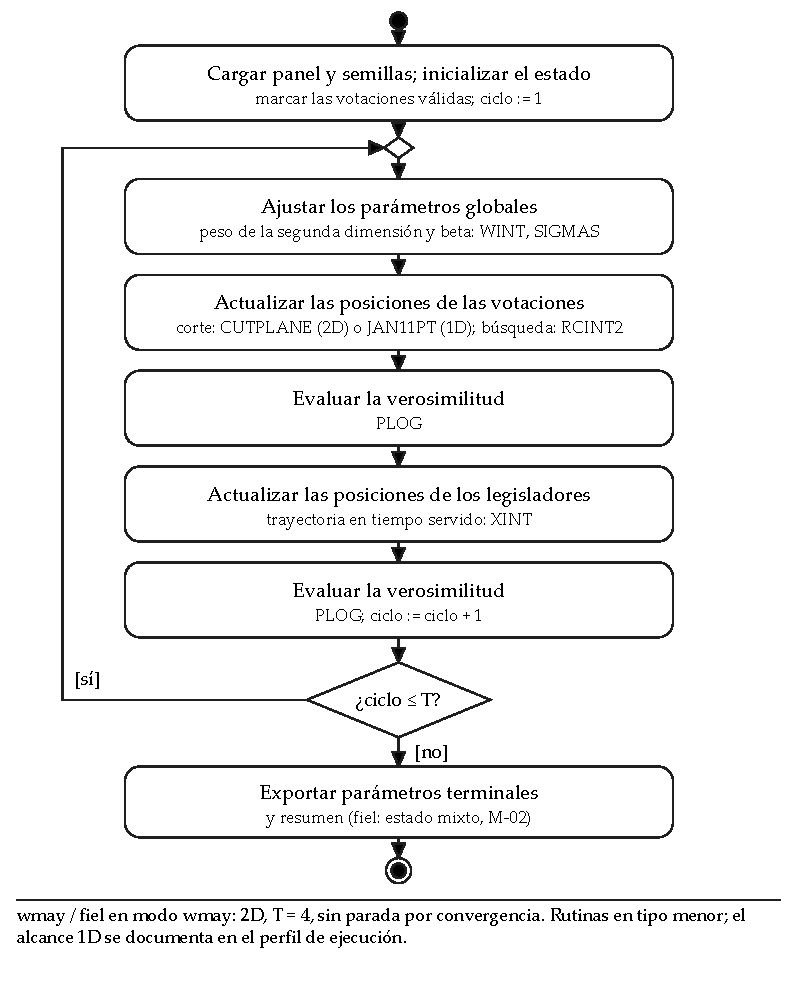
\includegraphics[width=13.5cm]{F4-ciclo-estimacion.pdf}}
\caption[F4. Actividad de estimación]{Actividad del perfil wmay/fiel: 2D, cuatro ciclos, parámetros terminales y resumen fiel mixto (M-02). No establece equivalencia con el original 2004.}
\label{fig:F4}
\end{figure}

\subsection{Intervención moderna}
\label{sec:T5}

¿Qué búsqueda cambia en cada actualización? El cuadro \ref{tab:T5} compara mecanismos
de implementación. El moderno conserva el modelo temporal y reemplaza búsquedas heredadas
por BOBYQA escalar \parencite{powell2009bobyqa} y COBYLA de bloques
\parencite{powell1994cobyla}, mediante NLopt \parencite{johnson_nlopt}. El perfil seleccionado
usa intervalos escalares locales y restricciones de norma; SLSQP y estrategias híbridas son
opciones fuera de ese perfil. Son implementaciones separadas (D-11, D-12).

El perfil de replicación fija la tabla de verosimilitud de la referencia y retira las cotas
globales de $w_2$ y $\beta$; persiste el intervalo local, y el portal añade precisión estricta
(D-13, D-25). La aceptación de bloques y el control de descenso global también son mecanismos
propios del moderno (D-32): el perfil no vuelve idénticos los recorridos de búsqueda. Panel,
semillas, ciclos y evaluación son controles del experimento, descritos en el cuadro
\ref{tab:protocolos} y el anexo \ref{anexo:perfil}. Esta intervención numérica es distinta
de la futura optimización de memoria con salidas idénticas; sus diferencias no se califican
automáticamente como errores de traducción.

\begin{table}[tbp]
\centering
\makebox[\textwidth][c]{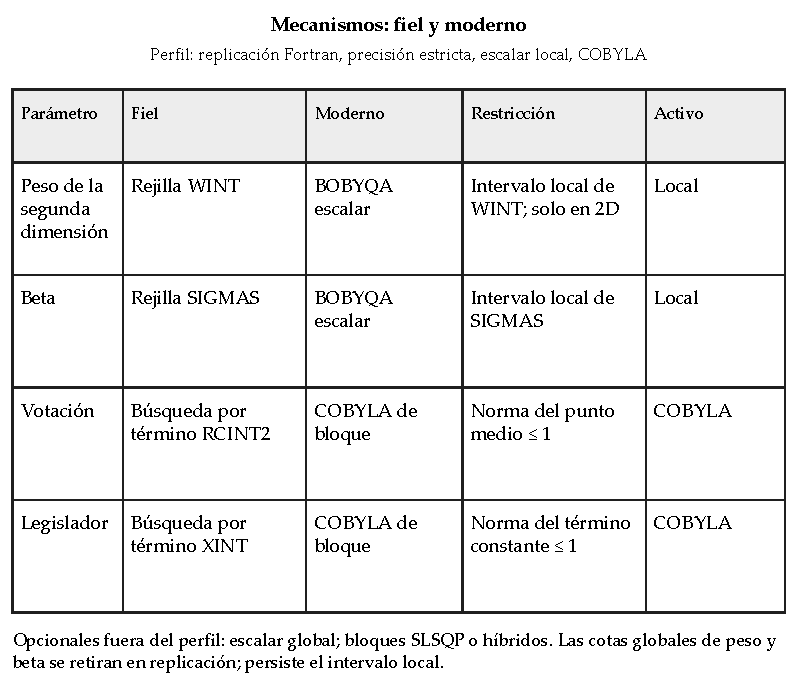
\includegraphics[width=13.5cm]{T5-mecanismos-modernos.pdf}}
\caption[T5. Mecanismos de la intervención moderna]{Mecanismos fieles y modernos en el perfil
controlado, verificados contra la implementación (D-13, D-25, D-32).}
\label{tab:T5}
\end{table}

\subsection{Datos y tiempo servido}
\label{sec:F6}

¿Qué significa cada fila y cómo se reconstruyen sus coordenadas? En la figura \ref{fig:F6}, un
legislador tiene una fila servida por periodo presente, con sus celdas de voto. Hay dos
contratos de semilla: el archivo por legislador, que el binario exige aunque cada legislador
pueda faltar en él, y el archivo por fila, opcional y con prioridad; sin ninguna, el
legislador parte del origen, como en la referencia, porque el origen es neutral (D-26). El
portal rechaza sembrar en proceso un panel de varios periodos, que dejaría en el origen a
quien no sirvió en el primero (D-27), y la comparación con wmay usa la semilla por
legislador, único contrato que esa referencia acepta. La trayectoria se evalúa solo en los
periodos servidos, con un tiempo local, y su grado efectivo es el de la regla de la referencia
(D-06): por eso el legislador del ejemplo, con dos periodos, recibe las mismas coordenadas en
sus dos filas. Como la escala de tiempo es propia de cada legislador, se exportan las
coordenadas en los periodos servidos y no sobre una rejilla global (D-10).

\begin{figure}[tbp]
\centering
\makebox[\textwidth][c]{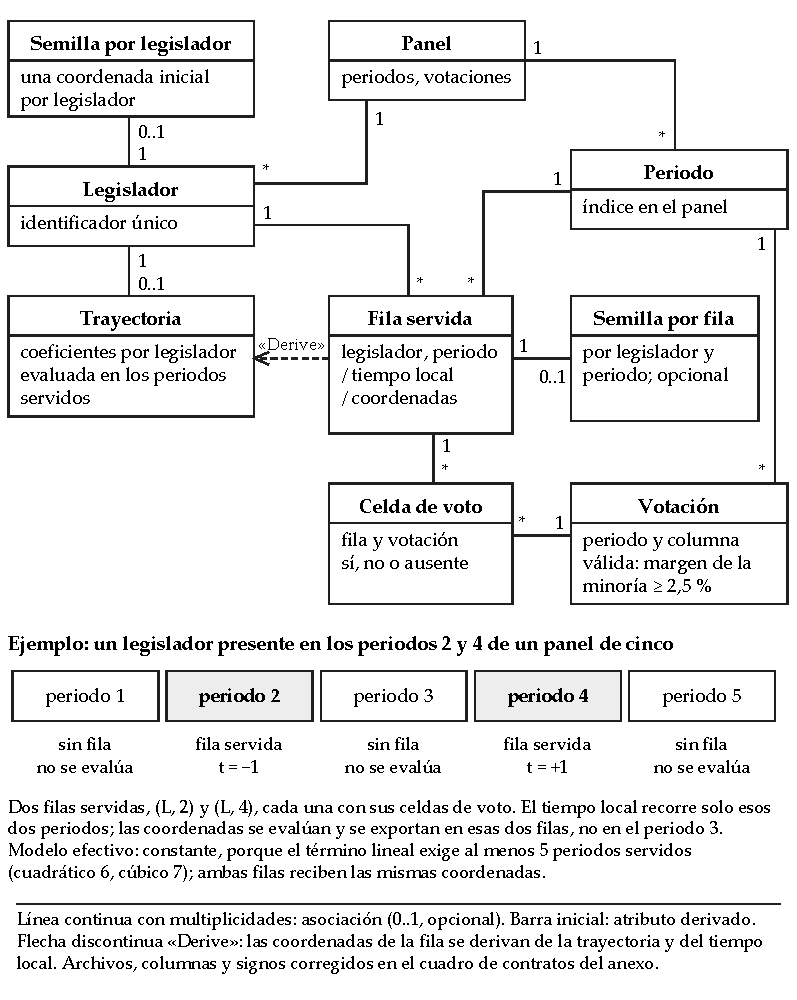
\includegraphics[width=13.5cm]{F6-datos-tiempo-servido.pdf}}
\caption[F6. Datos y tiempo servido]{Modelo conceptual de panel, filas servidas, semillas y trayectoria. El grado efectivo depende del número de periodos servidos (D-06, D-10, D-27).}
\label{fig:F6}
\end{figure}

\subsection{Proceso de verificación}
\label{sec:F7}

¿Qué comprobación permite confiar en la reimplementación y qué limita esa conclusión? La
figura \ref{fig:F7} muestra dos de los tres niveles de RF08 sobre corridas controladas, con el
mismo panel, la semilla por legislador y el mismo horizonte; el de componente está en el
cuadro \ref{tab:niveles}. (a) El estado terminal C++ se evalúa con la verosimilitud de wmay,
con cero ciclos, y se compara con la que la corrida wmay escribe en su resumen. (b) Las
coordenadas se emparejan por (legislador, periodo), se centran y se alinean por una
transformación ortogonal, rotación o reflexión, sin reescalar, y se informan las filas
emparejadas, las correlaciones por dimensión $r_1$ y $r_2$, la razón de amplitud $A$ (ecuación
\ref{eq:amplitud}) y la distancia media, con cobertura y marco. Es verificación, no validación
\parencite{oberkampf2010verification}; la amplitud acompaña a la correlación, invariante a la
escala \parencite{herron2004scale}, y el informe (RF09) añade el desacuerdo por votación
(D-14). Ninguna operación demuestra igualdad ni reemplaza
el control de paridad de entradas, documentado en el anexo \ref{anexo:perfil}; esta vista
usa wmay. El protocolo de aceptación de la tesis se declara por separado a continuación.

\begin{figure}[tbp]
\centering
\makebox[\textwidth][c]{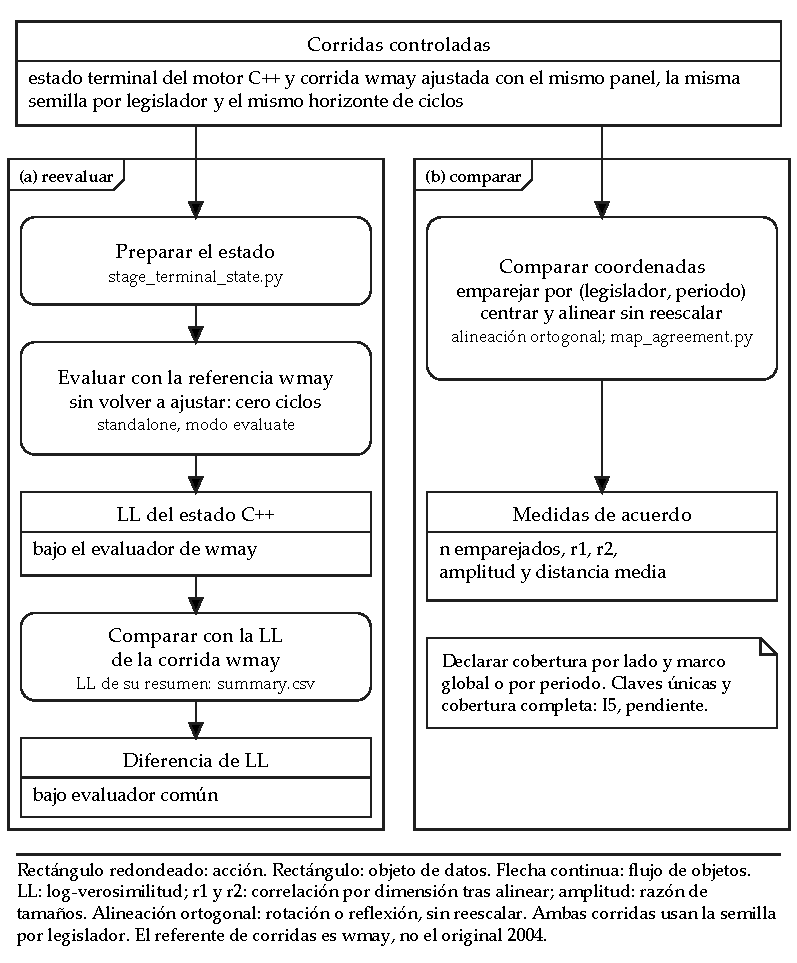
\includegraphics[width=13.5cm]{F7-verificacion.pdf}}
\caption[F7. Verificación con wmay]{Puntuación de estado y comparación de mapas del protocolo wmay. Cobertura y marco explícitos, alineación ortogonal sin reescalar (D-14).}
\label{fig:F7}
\end{figure}

\section{Decisiones de diseño y su razón}
\label{sec:decisiones}

El cuadro \ref{tab:decisiones} reúne las decisiones que explican las vistas, con la
alternativa descartada, la razón y la línea de código o configuración que la sostiene,
releída para este informe; las existentes conservan su número de la tesis y las nuevas siguen
desde D-22. El registro completo está en el anexo \ref{anexo:decisiones}, y la sección
\ref{sec:registros} lo agrupa en registros de decisión. Las rutas remiten al repositorio del
motor (\href{run:../evidence/engine/README.md}{motores, revisión ad945a9}) y al portal
(\href{run:../evidence/research/reproduce/R/dwnom.R}{portal en R}).

{\scriptsize
\setlength{\tabcolsep}{2pt}
\begin{longtable}{L{0.85cm}L{3.1cm}L{2.2cm}L{3.2cm}L{2.25cm}L{0.95cm}}
\caption[Decisiones de diseño que explican las vistas.]{Decisiones de diseño que explican las
vistas. Evidencia: F, \archivo{engines/faithful}; M, \archivo{engines/modern}; R,
\archivo{reproduce/R/dwnom.R}, con números de línea.}\label{tab:decisiones}\\
\toprule
Id & Decisión & Alternativa descartada & Razón & Evidencia & Figura \\
\midrule
\endfirsthead
\multicolumn{6}{l}{\scriptsize\emph{Cuadro \ref{tab:decisiones}, continuación}}\\
\toprule
Id & Decisión & Alternativa descartada & Razón & Evidencia & Figura \\
\midrule
\endhead
\bottomrule
\endfoot
D-22 & estado en \texttt{DWNominate}, trazado miembro a miembro a \texttt{xxcom\_mod}; fases
como métodos en orden & objetos por fase & la verificación por componente detiene el motor
entre fases y compara arreglos con la referencia & F \archivo{dwnominate.hpp:5-8} & F3, A1 \\
D-23 & búsquedas como funciones libres, contexto por argumento & métodos del orquestador & una
búsqueda sin estado propio se prueba aislada & F \archivo{grid_optimizer.hpp:126-151}; M
\archivo{tests/} & F3, A1 \\
D-24 & \texttt{GRID} de 2004 tras un interruptor que apaga \archivo{--wmay-replication} & un
solo linaje & comparar ambas fuentes sin cambiar el resto del optimizador & F
\archivo{dwnominate.hpp:55-59, 73}; R 252, 365 & F3, A2 \\
D-01 & SVD con \texttt{DGESDD}, la de wmay; sin LAPACK no se construye & Eigen sustituido en
silencio & la ruta de SVD mueve los óptimos de paneles dinámicos en cientos de nats & F
\archivo{CMakeLists.txt:22-30, 62-68} & F3 \\
D-31 & \texttt{std::sort} por índices y espectral de Eigen, no \texttt{RSORT}, \texttt{RS} ni
\texttt{DSYEV} & port literal & simplicidad, con el umbral de \texttt{REGA}; riesgo: otro orden
de empates & F \archivo{sort_utils.hpp:9-12}, \archivo{simple_ols.hpp:9-12} & F3 \\
D-07 & ciclos fijos sin prueba de convergencia; en el moderno, parada opcional apagada & regla
de parada común & la referencia no tiene criterio de convergencia; se compara a igual
horizonte & F \archivo{dwnominate.cpp:446}; M \archivo{main_cli.cpp:119-122} & F4, T5 \\
D-03 & sin reducción de punto flotante en regiones paralelas; suma en orden de índice &
reducción de OpenMP & otro orden de suma movía los bits bajos e invertía cuasiempates & F
\archivo{likelihood.cpp:423-433} & F4 \\
D-28 & el portal fija \archivo{OMP_NUM_THREADS}; un hilo para Fortran y fiel & hilos del
entorno & antes de D-03, hilos libres dispersaban 29,75 nats; hoy, número declarado y sellado & R 263, 329-336 &
F4, A2 \\
D-11, D-12 & búsquedas NLopt solo en el moderno; motores comparados, no
combinados & NLopt en el fiel; elegir un motor & fidelidad y mejora se responden con motores
distintos & árboles F y M & T5 \\
D-25 & perfil de replicación: tabla de verosimilitud de la referencia, sin cotas globales de
$w_2$ y $\beta$; el portal añade precisión estricta & opciones por omisión & aislamiento
causal: solo cambian las búsquedas & M \archivo{main_cli.cpp:379-390},
\archivo{dwnominate.cpp:569-573}; R 362-364 & T5 \\
D-13 & escalares del moderno en un intervalo local recentrado & caja global & conserva el
alcance de \texttt{SIGMAS} y \texttt{WINT} & M \archivo{parameter_optimizer.hpp:39-42} & T5 \\
D-32 & el moderno aborta si la LL previa es finita y $\Delta\ell<-10^{-8}$ & seguir y exportar &
inferencia: detectar una violación del contrato de bloque & M \archivo{dwnominate.cpp:384-393} & T5 \\
D-06 & grado efectivo: lineal con cinco periodos servidos, cuadrático con seis, cúbico con
siete & grado uniforme & es la regla de la referencia & F \archivo{dwnominate.cpp:1503-1511};
\archivo{wmay.f:1723} & F6 \\
D-10 & exportar en el tiempo normalizado de cada legislador & rejilla global & es donde
optimiza el motor & F \archivo{main_cli.cpp:435-436} & F6 \\
D-26 & sin semilla, el legislador parte del origen & rampa según el padrón & el origen es
neutral; la rampa inyectaba el orden de los identificadores & F
\archivo{csv_loader.cpp:570-609} & F6 \\
D-27 & el portal no siembra en proceso un panel de varios periodos & sembrar con el primer
periodo & dejaría en el origen a quien no sirvió en él, como a 61 de 168 senadores & R 286-299
& F6 \\
D-14 & tres niveles de verificación con evaluador común & coincidencia de salidas & un defecto
de indexación dejó igual la primera dimensión y alejó la verosimilitud &
\archivo{stage_terminal_state.py}, \archivo{map_agreement.py} & F7 \\
D-29 & salida cero, CSV requeridos legibles y directorio inicialmente vacío; excluidos devueltos
& leer lo que haya & rechaza archivos faltantes o previos; no valida toda la cobertura & R 279, 380-391
& A2 \\
D-30 & sello: binario y md5, SVD, hilos, semilla y md5, ciclos, banderas & confiar en la
documentación & hay binarios que no informan su SVD, que pesa más que el mayor desacuerdo entre
motores & R 27-30, 201-207 & F1, A2 \\
\end{longtable}
}

\section{Atributos de calidad: mecanismo y evidencia}
\label{sec:atributos}

El cuadro \ref{tab:atributos} lleva cada atributo de calidad que motiva la reimplementación al
mecanismo que lo persigue y a su evidencia; ninguno se da por demostrado. El rendimiento no se
ha medido todavía, y la carrera P-01 impide afirmar propiedad alguna del motor fiel con más
de un hilo hasta que se corrija.

\begin{table}[tbp]
\centering
\caption{Atributos de calidad: mecanismo de diseño, evidencia y estado.}
\label{tab:atributos}
\footnotesize
\begin{tabular}{L{2.7cm}L{4.2cm}L{2.4cm}L{3.0cm}}
\toprule
Atributo & Mecanismo & Evidencia & Estado \\
\midrule
Mantenibilidad y auditabilidad (RNF09) & configuración explícita; cabeceras por
responsabilidad, dependencias acíclicas; correspondencia uno a uno con la referencia;
desviaciones registradas & F3, A1; D-19, D-22, D-23, D-31 & criterio de diseño; no medido \\
\addlinespace
Operabilidad (RNF03, RNF06) & un portal común a las tres variantes; aceptación con salida cero
y CSV requeridos legibles; excluidos devueltos; sello & F1, A2; D-27
a D-30; anexo \ref{anexo:construccion} & en uso; reejecución desde un clon limpio pendiente
(F1 del backlog) \\
\addlinespace
Rendimiento (RNF04) & paralelismo por votación y legislador; comparación a un hilo; mejora
aceptada solo con resultados idénticos & F4; D-03, D-20, D-21, D-28 & \textbf{no medido}; con
más de un hilo, bloqueado por P-01 \\
\addlinespace
Fidelidad y reproducibilidad (RNF01, RNF02) & \texttt{DGESDD}, aritmética estricta,
\texttt{GRID} apagado, perfil de replicación; ciclos igualados; tres niveles de verificación &
F3, T5, F7; D-01, D-02, D-07, D-14, D-24, D-25 & umbral pendiente del propietario; sin caso de
prueba por hilos \\
\addlinespace
Portabilidad (RNF05) & C++ estándar con CMake; dependencias que detienen la construcción si
faltan; sin código específico de la máquina & D-01, D-02; anexo \ref{anexo:construccion} &
clon limpio en la Etapa 4 \\
\bottomrule
\end{tabular}
\end{table}

\section{Diseño que las figuras no sustituyen}
\label{sec:cuadros}

\subsection{Verificación por niveles}
\label{sec:niveles}

El cuadro \ref{tab:niveles} completa los tres niveles de RF08 con su referente. La
inicialización por mínimos cuadrados de los legisladores es la única rutina portada que el
nivel de componente aún no audita. El conjunto de falsación reintroduce un defecto real ya
corregido y exige que la decisión de aceptación lo rechace, no cada métrica aislada (D-15). Cuatro controles preceden a toda
comparación: paridad de entradas, determinismo por hilos, configuración igualada y tolerancia
declarada entre máquinas.

\begin{table}[tbp]
\centering
\caption{Los tres niveles de verificación de RF08: referente, mecanismo y medida.}
\label{tab:niveles}
\footnotesize
\begin{tabular}{L{2.0cm}L{1.7cm}L{2.8cm}L{3.2cm}L{2.3cm}}
\toprule
Nivel & Referente & Qué se compara & Mecanismo & Medida y aceptación \\
\midrule
Componente & original 2004; las pruebas unitarias, sin referente & cada rutina portada contra
el estado intermedio: dirección de corte, errores por votación, escalares del primer ciclo &
volcado de fases del fiel frente al registro por votación de 2004; en el moderno, bloques
fijados (\archivo{--fix-*}, \archivo{--evaluate-only}) y pruebas unitarias; el fiel declara
esos modos, pero su CLI los deja apagados & tablas por rutina a ciclos igualados; escalares
idénticos tras el primer ciclo \\
\addlinespace
Estado & wmay & la verosimilitud de un estado terminal bajo un único evaluador & estado
preparado; wmay en modo \texttt{evaluate}, cero ciclos & $\ell/N$ y desacuerdo por votación;
umbral $\tau$ por fijar \\
\addlinespace
Mapa & wmay & dos configuraciones emparejadas por (legislador, periodo) & alineación ortogonal
sin reescalar, en marco global y por periodo & $r_1$, $r_2$, $A$, distancia, reflexiones;
cláusulas por fijar (D-15) \\
\bottomrule
\end{tabular}
\end{table}

\subsection{Referentes y protocolos de comparación}
\label{sec:protocolos}

La indicación del 5 de octubre fue comparar con el Fortran original (00:54:23); el profesor
guía no identificó un hash en esa conversación. Los autores la vinculan a la distribución
2004 y al ejecutable reconstruido registrado en el anexo \ref{anexo:procedencia}. Se separan
dos protocolos, porque la referencia del artículo JCC2026 es wmay en sus brazos estáticos y
dinámicos. No se reinterpretan los resultados publicados como resultados de 2004.

\begin{table}[tbp]
\centering
\caption{Protocolos de referencia y alcance de sus medidas.}
\label{tab:protocolos}
\footnotesize
\begin{tabular}{L{2.4cm}L{4.8cm}L{5.2cm}}
\toprule
Propósito & Brazos y configuración & Evaluación y límite \\
\midrule
Reproducción del artículo & wmay y fiel en modo wmay: DGESDD, GRID apagado;
moderno como intervención controlada & puntuación común con wmay (F7), mapas y LL nativa
identificada; no constituye aceptación contra 2004 \\
\addlinespace
Aceptación de tesis E3/E4 & original 2004 (LSVRR, GRID) y fiel con GRID activo;
documentar DGESDD y desviaciones D-19 & mismos paneles, orden, semillas y precisión;
estado, mapas y LL nativa por evaluador. Puntuar ambos con wmay es un control adicional \\
\addlinespace
Rendimiento & original 2004 como referencia externa; fiel antes/después de cada
cambio de memoria & un núcleo, misma máquina, entradas y ciclos; builds y banderas
comparables. La regresión exige salidas idénticas del fiel \\
\bottomrule
\end{tabular}
\end{table}

El modo \archivo{faithful2004-safeguard} conserva GRID, pero no acredita equivalencia de todo
el motor: SVD, exportación y desviaciones deben registrarse. Las comparaciones original/wmay
retenidas del 6 de octubre establecen acuerdo cercano bajo semillas comunes redondeadas;
las recompilaciones reprodujeron cada salida estadounidense propia. No son una medición de
velocidad ni demuestran igualdad entre motores. El umbral RNF01 y su ratificación siguen
pendientes; E2 especifica el protocolo, E3/E4 lo ejecutan.

\subsection{Diseño experimental de las pruebas exhaustivas}
\label{sec:experimental}

Las pruebas exhaustivas de la Etapa 4 establecen, para cada panel de un conjunto fijado de
antemano, si el motor fiel satisface el protocolo original 2004 dentro de la tolerancia de RNF01
\parencite[cap.~5, §2.2.1]{swebok2025}. El diseño, escrito antes de correrlas (tarea H8),
fija paneles, estadísticos de los tres niveles, identidad de las salidas numéricas con uno, dos, cuatro y
doce hilos, y ajustes igualados (anexo \ref{anexo:paneles}). El umbral se propone en su forma:
un $\tau$ sobre la diferencia de verosimilitud por voto, que a diferencia de la absoluta viaja
entre paneles de tamaño distinto, más dos cláusulas de mapa que el conjunto de falsación mostró
sensibles a un defecto real, cada una entre el valor de una versión defectuosa y el de una
corregida (D-15). El valor es decisión del propietario; el piso de ruido de la configuración
igualada, que se medirá en la Etapa 3, lo acota desde abajo.

\subsection{Mejora de rendimiento del motor fiel}
\label{sec:rendimiento}

En la comparación publicada, a un hilo, el motor fiel es más lento que wmay en seis de siete
paneles \parencite{nieves2026jcc}, y el propietario pidió alcanzar el rendimiento a un núcleo
del original 2004 revisando punteros y estructuras de datos. La comparación publicada con
wmay es antecedente; el referente externo de E3/E4 es el original 2004 del cuadro
\ref{tab:protocolos}. Se diseña como prueba de regresión más
prueba de rendimiento \parencite[cap.~5, §2.2.5 y §2.2.7]{swebok2025}; nada está implementado
ni se anticipa magnitud alguna. La hipótesis, que el perfilado debe contrastar, es que el
tiempo se va en recorrer celdas vacías: los votos se guardan con una fila por legislador y
periodo y una columna por votación del panel entero. Los cambios candidatos restringen los
lazos al bloque de cada periodo, guardan los votos contiguos y suprimen trabajo sin efecto en
el resultado (M-01 a M-09). Se acepta un cambio solo si las salidas son idénticas a uno y a
varios hilos (D-20); el protocolo corrige antes P-01, reconstruye la línea base, perfila,
repite corridas intercaladas y aplica los cambios de a uno (D-21; anexo
\ref{anexo:rendimiento}).

\subsection{Diseño del estudio chileno: bootstrap y periodización}
\label{sec:algoritmos}

El estudio chileno, que la sección \ref{sec:propuesta-chile} propone leer como la validación
en condiciones operativas reales, estima el desplazamiento de las medianas de partido en la
primera dimensión durante el 55.º periodo legislativo, con cortes fijados desde el calendario e
inferencia por bootstrap paramétrico \parencite{lewis2004measuring,carroll2009measuring} con
valores iniciales regenerados en cada réplica y ajuste de \textcite{holm1979simple} (RF10,
RF11; algoritmo \ref{alg:bootstrap}). La periodización, que mueve el resultado (RF12), se trata
como parámetro declarado (tarea E3): el diseño principal, pendiente de ratificación (D-16), es
una ventana igualada de doce unidades de cuatro meses en un marco, con tres diseños de
sensibilidad y una regla de discretización de tres cláusulas; la inferencia se hace solo en la
primera dimensión (D-17). El diseño completo, con el cuadro de periodizaciones, está en el
anexo \ref{anexo:chile}.

\subsection{Trazabilidad de los requisitos funcionales al diseño}
\label{sec:trazabilidad}

El cuadro \ref{tab:traza} asigna cada requisito funcional al elemento de diseño que lo
satisface, con lo que queda a la implementación \parencite[cap.~11, §3.4]{swebok2025}, como
revisión del diseño contra los requisitos \parencite[cap.~3, §6.5]{swebok2025}; los no
funcionales están en el cuadro \ref{tab:atributos}.

\begin{table}[tbp]
\centering
\caption{Trazabilidad entre requisitos funcionales y elementos de diseño.}
\label{tab:traza}
\footnotesize
\begin{tabular}{L{1.5cm}L{6.6cm}L{4.3cm}}
\toprule
Req. & Elemento de diseño (dónde se ve) & Pendiente \\
\midrule
RF01, RF02 & validación en la carga y en el portal; dos contratos de semilla (F6, A2; D-26,
D-27) & filas cortas, identificadores no numéricos, códigos fuera de rango (A4) \\
RF03, RF04 & misma maquinaria para uno o varios periodos (F4, F6; D-06) & sin brecha de diseño; pruebas E3 \\
RF05 & módulos uno a uno con la referencia; dos linajes (F3, A1; D-22 a D-24) & ninguno \\
RF06 & variante en las cuatro búsquedas; perfil de replicación (T5; D-25) & registrar la SVD en
el resumen del moderno \\
RF07 & marco de exportación declarado (F6; D-10) & A5; resumen y exportación 1D (I2) \\
RF08, RF09 & tres niveles; desacuerdo por votación (F7; cuadro \ref{tab:niveles}; D-14) &
OLS; modos de componente (I4); claves y productor RF09 (I5) \\
RF10, RF11 & bootstrap con semillas regeneradas, Holm, elegibilidad (alg. \ref{alg:bootstrap})
& brazo fiel sobre el diseño principal \\
RF12 & periodización declarada (cuadro \ref{tab:disenos}; D-16) & rejilla de igual recuento \\
\bottomrule
\end{tabular}
\end{table}

\chapter{Documenta adecuadamente el proyecto}
\label{cap:documentacion}

Este capítulo reúne la documentación que respalda el desarrollo: los registros de decisión de
diseño, los cambios implementados en esta etapa con las desviaciones declaradas respecto del
plan original, y la evidencia de los repositorios git con su convención de mensajes.

\section{Registros de decisiones de diseño}
\label{sec:registros}

El registro tiene treinta y dos decisiones: D-01 a D-21, fechadas al 2 de octubre de 2026 en
el documento de tesis, y D-22 a D-32, agregadas en esta etapa al releer el código (anexo
\ref{anexo:decisiones}). Los nueve registros siguientes agrupan las significativas, las
costosas de revertir \parencite[cap.~2, §2.4]{swebok2025}, con la fundamentación que pide
SWEBOK \parencite[cap.~3, §4.6]{swebok2025}; la razón y la evidencia de cada decisión están en
el cuadro \ref{tab:decisiones}.

\begingroup
\setbeforeparaskip{-1ex}
\paragraph{RD-1. Motores (D-11, D-12, D-25).} Para auditar el estimador y aislar la mejora,
se separan port y NLopt. Se descartan paquetes R y estimadores bayesianos
\parencite{clinton2004statistical,martin2002dynamic,shin2025l1ideal}; Fortran sigue como oráculo. Vigente.

\paragraph{RD-2. Organización (D-19, D-22--D-24, D-31).} Trazar arreglos exige estado
concentrado y búsquedas libres; GRID es configurable. Se descartan objetos por fase y un
único linaje, sin afirmar ocultamiento completo. Vigente.

\paragraph{RD-3. Configuración (D-01, D-02).} Una SVD sustituida invalidó la reproducción.
El perfil wmay/fiel fija DGESDD y aritmética estricta: se descartan sustitución automática
y \emph{fast-math}; otra configuración requiere otro sello. Vigente.

\paragraph{RD-4. Hilos (D-03, D-28).} El acumulador compartido dispersaba corridas:
suma ordenada y comparación a un hilo, sin reducciones flotantes OpenMP. Las pruebas
manuales no cierran P-01; I1 exige corrección y prueba 1/2/4/12. Vigente, corrección pendiente.

\paragraph{RD-5. Ciclos (D-07, D-32).} Sin convergencia declarada, se comparan ciclos
iguales; se descarta una parada común. El moderno controla el descenso mediante su propio
mecanismo. Vigente.

\paragraph{RD-6. Portal (D-08, D-10, D-26--D-30).} Las banderas divergían entre llamadas:
un contrato R impone aceptación, excluidos, sello y tiempo servido, sin migrar todos los
guiones. Sin sello se regenera; los hilos faltan en el resumen fiel (P-02). Vigente.

\paragraph{RD-7. Verificación (D-14, D-15).} Un error apenas movió D1 y sí la
verosimilitud \parencite{nieves2026jcc}: se exige componente, estado, mapa y falsación,
descartando solo salidas finales o umbrales de corridas que pasan. Vigente; umbral pendiente.

\paragraph{RD-8. Chile (D-16, D-17).} Periodización y D2 afectan los resultados
\parencite{nieves2026jcc}: ventana igualada e inferencia en D1, frente a ventana expansiva
y ambas dimensiones. D-16 por ratificar; D-17 vigente.

\paragraph{RD-9. Rendimiento (D-20, D-21).} La desventaja frente a wmay
\parencite{nieves2026jcc} motiva medir contra el original 2004 y contra sí mismo. Se exige
salida fiel idéntica; se descartan tolerancias y tiempos publicados como base. E3 propuesto;
P-01 primero.
\endgroup

\section{Cambios implementados y desviaciones declaradas}
\label{sec:cambios}

Los cambios de esta etapa son de diseño y de documentación; no se implementó código nuevo en
los motores, que existen desde el trabajo del artículo con el banco de verificación y el
paquete de reproducción. El cuadro \ref{tab:cambios-etapa} los registra con fecha y razón, y
el cuadro \ref{tab:desviaciones} declara las desviaciones respecto del plan original.

\footnotesize
\begin{longtable}{L{1.4cm}L{7.0cm}L{4.2cm}}
\caption{Cambios implementados en la Etapa 2.}\label{tab:cambios-etapa}\\
\toprule
Fecha & Cambio & Por qué \\
\midrule
\endfirsthead
\multicolumn{3}{l}{\footnotesize\emph{Cuadro \ref{tab:cambios-etapa}, continuación}}\\
\toprule
Fecha & Cambio & Por qué \\
\midrule
\endhead
\bottomrule
\endfoot
10 sep. & registro de tareas retirado del documento de tesis & vive en la planilla \\
24 sep. & capítulo 4, Diseño, y Anexo A, Registro de diseño & entregable de diseño \\
2 oct. & capítulo 2 completado; capítulo 4 revisado (atributos de calidad, mejora de
rendimiento, D-20, D-21); cifras corregidas & indicación del 28 sept.; auditoría de cifras \\
4 oct. & revisión adversarial independiente: 31 hallazgos, 28 corregidos y 2 en parte; RNF09 &
control de calidad \\
5 a 8 oct. & juego de auditoría de nueve vistas; figuras F1 a F4, F6, F7, A1 y A2 y cuadro T5, corregidos tras una
revisión independiente; D-22 a D-32; cuadros de atributos, niveles, construcción, errores y
perfil; este informe & indicaciones del 5 oct.; ningún pie daba la razón de una decisión \\
\end{longtable}

\begin{longtable}{L{2.6cm}L{5.3cm}L{4.7cm}}
\caption{Desviaciones respecto del plan original y su justificación.}\label{tab:desviaciones}\\
\toprule
Desviación & Qué cambió & Por qué \\
\midrule
\endfirsthead
\multicolumn{3}{l}{\footnotesize\emph{Cuadro \ref{tab:desviaciones}, continuación}}\\
\toprule
Desviación & Qué cambió & Por qué \\
\midrule
\endhead
\bottomrule
\endfoot
Entregable & informe propio por criterio & acuerdo del 5 de octubre \\
Planificación & E3 y H8 adelantadas a la Etapa 2; H1 a H9 agregadas & todo el diseño se mide
al cierre de la Etapa 2 \\
Implementación & A4 y A5 no se iniciaron & el esfuerzo fue al diseño; se reprograman \\
Requisitos & RNF09 después de la Etapa 1 & el diseño se apoya en ese atributo \\
Plazo de OE1 & mejora completa medida a inicios de diciembre & alcanzable en el curso \\
Extensión de la tesis & el cuerpo pasó de 40 a 53 páginas y bajó a 50 & se reduce hacia la
Etapa 4 \\
Commits & Etapa 1 en un commit; desde la Etapa 2, uno por pasada & el criterio lee el
historial \\
Utilidad & sin el factor $1/2$ del artículo, declarado & reproduce las tres implementaciones;
la errata queda para sus autores \\
\end{longtable}
\normalsize

\section{Repositorios git y evidencia de commits}
\label{sec:git}

El cuadro \ref{tab:repos} excluye cambios sin commit. RNF08 exige
\texttt{área(ID): verbo y qué}, razón en el cuerpo y un commit por pasada del documento.
Portal y backlog se verificaron; sus estados difieren del registro de artefactos. Diseño y reorganización siguen locales
(anexo \ref{anexo:procedencia}). Publicación y planilla quedan pendientes.

\begin{table}[htbp]
\centering
\caption{Repositorios del proyecto y su actividad, medida el 8 de octubre de 2026.}
\label{tab:repos}
\footnotesize
\begin{tabular}{L{3.4cm}L{1.75cm}L{2.1cm}L{5.0cm}}
\toprule
Repositorio & Visibilidad & Commits desde 4 sept. & Observación y ejemplo de mensaje \\
\midrule
\href{https://github.com/cowerino/dwnominate-chile}{Motores y reproducción} &
público & 0 públicos; 6 locales & rama pública \archivo{00ba24c0}; reorganización local en \archivo{ad945a91} \\
\addlinespace
\href{https://github.com/quevotan/quevotan-db/commits/fc25b1c9302cfd7b35a265357c203f21848983b6}{Investigación y backlog} &
privado, del equipo & 37 remotos, sin fusiones & \archivo{0ab30d3}: corrige formatos de semillas y documenta ajustes fallidos \\
\addlinespace
Documento de tesis e informes & privado & 8 locales & \archivo{40dae6b}: corrige diseño contra fuentes; esta revisión sigue sin commit \\
\bottomrule
\end{tabular}
\end{table}


\FloatBarrier
\clearpage
\renewcommand{\clearforchapter}{\clearpage}
\printbibliography

\appendix
\chapter{Figuras y algoritmos de detalle}
\label{anexo:figuras}

Este anexo da la notación del modelo, los dos algoritmos que el cuerpo resume, el ciclo de
estimación del motor fiel (vista F4) y el bootstrap paramétrico del estudio chileno, y las dos
vistas de detalle. En el algoritmo \ref{alg:ciclo}, tres reglas son decisiones de diseño: el
grado efectivo se fija por legislador (D-06); el tiempo se normaliza sobre los periodos
servidos (D-10); y las constantes de las búsquedas se toman de la referencia y se declaran en
la configuración de cada módulo. Dos desviaciones conocidas se declaran (D-19): las búsquedas
escalares restauran al salir el mejor estado observado, donde el bucle original puede terminar
en un paso no evaluado, y una restricción de separación que en la referencia es código
inalcanzable no se porta.

La figura \ref{fig:A1} muestra quién posee el estado del motor fiel. CSVLoader crea la
entrada; DWNominate copia de ella en el constructor lo que necesita (votos, coordenadas,
puntos medios y dispersiones) y no retiene el objeto de entrada; posee por valor la
configuración, los metadatos de periodos y la presencia de legisladores, usa las búsquedas
como funciones libres (D-23) y crea el resultado, con el estado terminal, al terminar (D-22).
La CLI construye la configuración y deja apagados sus tres modos de validación, que fijan un
bloque de parámetros; solo el motor moderno los expone como banderas. El interruptor de la
salvaguarda \texttt{GRID} de 2004 está encendido por omisión y \archivo{--wmay-replication} lo
apaga (D-24).

La figura \ref{fig:A2} sigue una estimación con el motor fiel desde el portal en R. La CLI
carga y valida las entradas (inicialización: semillas, $\beta$ y $w_2$), crea el motor con la
configuración y los datos, llama una vez a \texttt{run()} y exporta parámetros terminales
y el resumen fiel mixto (M-02, pendiente de I2).
La nota apunta documentalmente a F4; no es un uso de interacción UML ni añade otro bucle. Solo la carga y la ejecución están dentro de
bloques de captura: si lanzan una excepción, la CLI termina con código 1 y sin salidas; la
construcción del motor y la exportación quedan fuera, y si un archivo de salida no se puede
abrir, la CLI lo omite y termina con código 0, de modo que es la comprobación de archivos del
portal la que rechaza la corrida. El portal acepta el
resultado solo si el código de salida es cero y las coordenadas, los parámetros y el resumen
se pueden leer (D-29), sin comprobar toda su cobertura o esquema. Sella la corrida (D-30);
con el modo wmay, que es el de omisión, añade
\archivo{--wmay-replication} (D-24). El paralelismo con OpenMP es una capacidad del motor; la
corrida comparativa usa un hilo (D-28).

\section*{Notación}
La notación es la del capítulo 2 del documento de tesis. El legislador $i$
ocupa el punto $\mathbf{x}_i$ en $s$ dimensiones; la votación $j$ tiene dos resultados,
$\mathbf{o}_j^{\mathrm{S}}$ y $\mathbf{o}_j^{\mathrm{N}}$, dados por su punto medio y su
separación, con utilidades y probabilidad de votar a favor
\begin{equation}
u_{ij}^{c} = \exp\Bigl(-\sum_{k=1}^{s} w_k^{2} \bigl(x_{ik} - o_{jk}^{c}\bigr)^{2}\Bigr),
\quad c \in \{\mathrm{S}, \mathrm{N}\},
\label{eq:util}
\end{equation}
\begin{equation}
\Pr\bigl(\mathrm{voto}_{ij} = \mathrm{S}\bigr) = \Phi\bigl(\beta \,[u_{ij}^{\mathrm{S}} - u_{ij}^{\mathrm{N}}]\bigr),
\label{eq:prob}
\end{equation}
con $w_1 = 1$, $w_2$ el peso de la segunda dimensión, $\beta$ el parámetro de señal y $\Phi$
la normal estándar. La log-verosimilitud $\ell$ suma el logaritmo de la probabilidad de cada
voto de las votaciones válidas, las de margen de la minoría ${\ge}\,2{,}5$\,\%, y $\ell/N$ es la
verosimilitud por voto. Dos
configuraciones se comparan centrándolas y alineando una con la otra por la transformación
ortogonal óptima, sin cambio de escala; se informan las correlaciones por dimensión $r_1$ y
$r_2$, la distancia media y la razón de amplitud
\begin{equation}
A = \mathrm{rms}(X)/\mathrm{rms}(X_{\mathrm{ref}}), \qquad
\mathrm{rms}(X) = \Bigl({\textstyle\frac{1}{n}} \sum_{i=1}^{n} \Vert \mathbf{x}_i - \bar{\mathbf{x}} \Vert^{2}\Bigr)^{1/2}.
\label{eq:amplitud}
\end{equation}


\begin{algorithm}[htbp]
\caption{Ciclo de estimación del motor fiel.}
\label{alg:ciclo}
\small
\begin{algorithmic}[1]
\Require matrices de votaciones $V$ de $I$ legisladores y $J$ votaciones, valores iniciales $X^{(0)}$, dimensiones $s$, grado $m$, ciclos $T$
\State $w \gets (1, w_2^{(0)}, \beta^{(0)})$; marcar válida cada votación con margen de la minoría ${\ge}\,2{,}5$\,\%
\For{$c = 1, \dots, T$}
  \If{$s \ge 2$} $w_2 \gets$ búsqueda local por pasos desde un paso de $0{,}01$ \EndIf
  \State $\beta \gets$ búsqueda local por pasos desde un paso de $0{,}1$
  \ForAll{votación válida $j$, en paralelo}
     \State proyectar el punto medio $\mathbf{z}_j$ a la bola unitaria
     \State calcular el plano de corte; si $c = 1$ y no hay parámetros precargados, tomar de él $(\mathbf{z}_j, \mathbf{d}_j)$ iniciales y con ellos la polaridad; en los ciclos siguientes, solo registrarlo
     \State $(\mathbf{z}_j, \mathbf{d}_j) \gets$ cinco rondas de búsqueda lineal alternada en separación y punto medio
  \EndFor
  \State evaluar la verosimilitud global
  \ForAll{legislador $i$ con al menos un periodo servido, en paralelo}
     \State grado efectivo según periodos servidos: constante con menos de cinco, lineal con cinco, cuadrático con seis, cúbico con siete o más, sin exceder $m$
     \State término constante inicial por mínimos cuadrados sobre las coordenadas vigentes (en el primer ciclo, los valores iniciales; con menos de cinco periodos, la del primero servido), reescalado a radio 0,75 si queda fuera de la bola
     \State optimizar el término constante con el legislador inmóvil y la restricción de la bola; luego cada término temporal, desde cero y con los anteriores fijos
     \State reconstruir las coordenadas por periodo sobre su tiempo normalizado
  \EndFor
  \State evaluar la verosimilitud global
\EndFor
\State \Return coordenadas, parámetros de votación, $w$, verosimilitud y estadísticos de clasificación
\end{algorithmic}
\end{algorithm}

\begin{algorithm}[htbp]
\caption{Bootstrap paramétrico de medianas de partido.}
\label{alg:bootstrap}
\small
\begin{algorithmic}[1]
\Require panel observado $V$; ajuste observado $(\hat X, \hat Z, \hat D, \hat\beta, \hat w_2)$, con $\hat Z$ y $\hat D$ el punto medio y la separación de cada votación; membresía $M(i,t)$; cortes $t_1 < t_2 < t_3$; réplicas $B$; estado maestro del generador aleatorio
\For{$b = 1, \dots, B$}
  \State derivar el generador aleatorio de la réplica desde el estado maestro
  \State fijar la máscara de redibujo desde el panel observado: celdas no ausentes, votaciones elegibles y separación no nula
  \ForAll{unidad $t$, diputado $i$, votación $j$ en esa máscara}
    \State $p \gets \Phi\!\left(\hat\beta\,(u^{\mathrm{S}}_{ij} - u^{\mathrm{N}}_{ij})\right)$, con las utilidades de la ecuación (\ref{eq:util}) evaluadas en el ajuste observado
    \State $V_b[i,j,t] \gets$ a favor con probabilidad $p$, en contra en otro caso
  \EndFor
  \State valores iniciales de la réplica: estimador estático por unidad sobre $V_b$, con signos armonizados
  \State $X_b \gets$ motor$(V_b)$ desde esos valores iniciales, con el mismo grado, dimensiones, regla y umbral de elegibilidad, ciclos y optimizador; recalcular las votaciones retenidas sobre $V_b$
  \State alinear $X_b$ a $\hat X$ en la primera dimensión por signo y localización
\EndFor
\State fijar las cohortes desde el ajuste observado y reutilizarlas sin cambio en cada réplica
\ForAll{cohorte $c$, partido $p$}
  \State $\delta \gets m_p(t_3) - m_p(t_1)$ sobre $\hat X$; \quad $\Delta_b \gets$ lo mismo sobre $X_b$; \quad $e_b \gets \Delta_b - \delta$
  \State cota superior básica $\gets \delta - q_\alpha(e)$; \quad cota superior percentil $\gets q_{1-\alpha}(\Delta)$
  \State $p_{\mathrm{izq}} \gets (1 + \#\{e_b \le \delta\})/(B+1)$; sesgo $\gets \bar\Delta - \delta$ junto al percentil
  \State elegible si el partido tiene al menos cinco miembros en $t_1$ y en $t_3$
\EndFor
\State ajustar $p_{\mathrm{izq}}$ por Holm dentro de cada familia (cohorte, par de cortes) sobre los partidos elegibles
\State \Return por (cohorte, partido): $\delta$, cotas, $p$ ajustado, indicador de robustez
\end{algorithmic}
\end{algorithm}

La máscara de redibujo observada no es la máscara de ajuste de la réplica. El generador
conserva las celdas fuera de ella; el motor moderno recalcula la proporción minoritaria en
$V_b$ y retiene votaciones según la misma regla y umbral. Una votación elegible observada puede
dejar de serlo en una réplica. Esto corrige la descripción, sin cambiar el bootstrap ni
atribuirle un daño numérico medido. Las semillas por periodo se regeneran y armonizan en cada
réplica; no se reutiliza el contrato de semilla común por legislador de los tres brazos.

\begin{figure}[htbp]
\centering
\makebox[\textwidth][c]{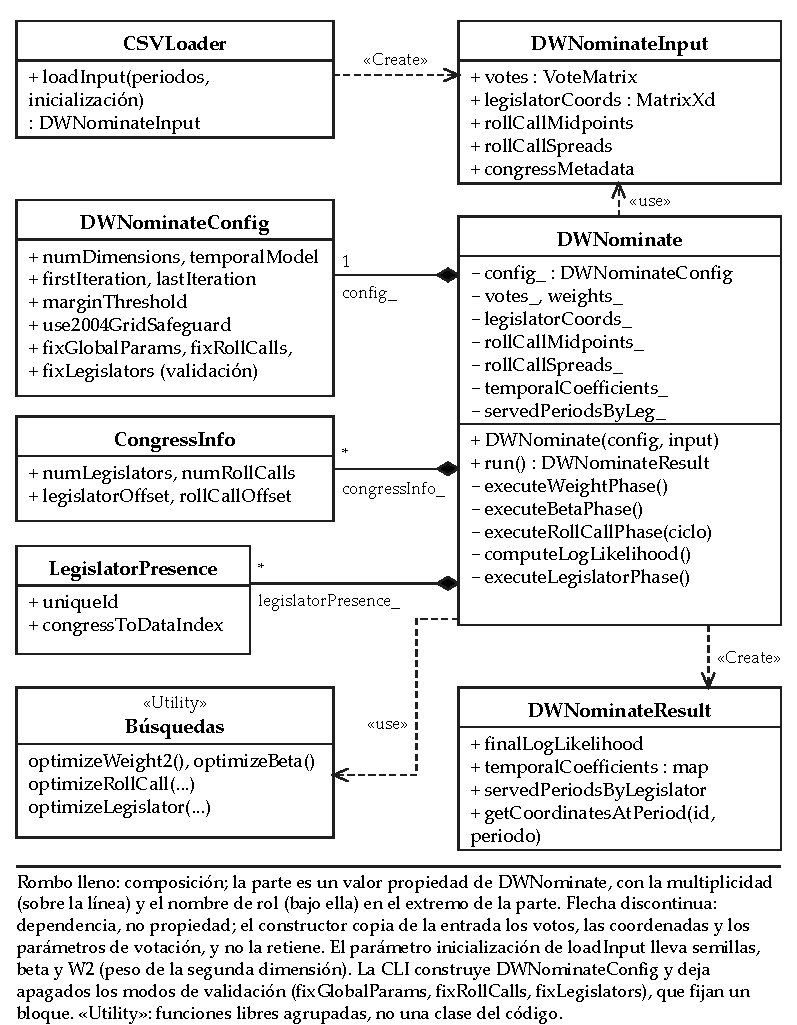
\includegraphics[width=13.5cm]{A1-clases-estado.pdf}}
\caption[A1. Clases y propiedad del estado del motor fiel]{Clases y propiedad del estado del
motor fiel: DWNominate posee la configuración y el estado numérico, usa búsquedas libres (D-23)
y crea el resultado con el estado terminal (D-22).}
\label{fig:A1}
\end{figure}

\begin{figure}[htbp]
\centering
\makebox[\textwidth][c]{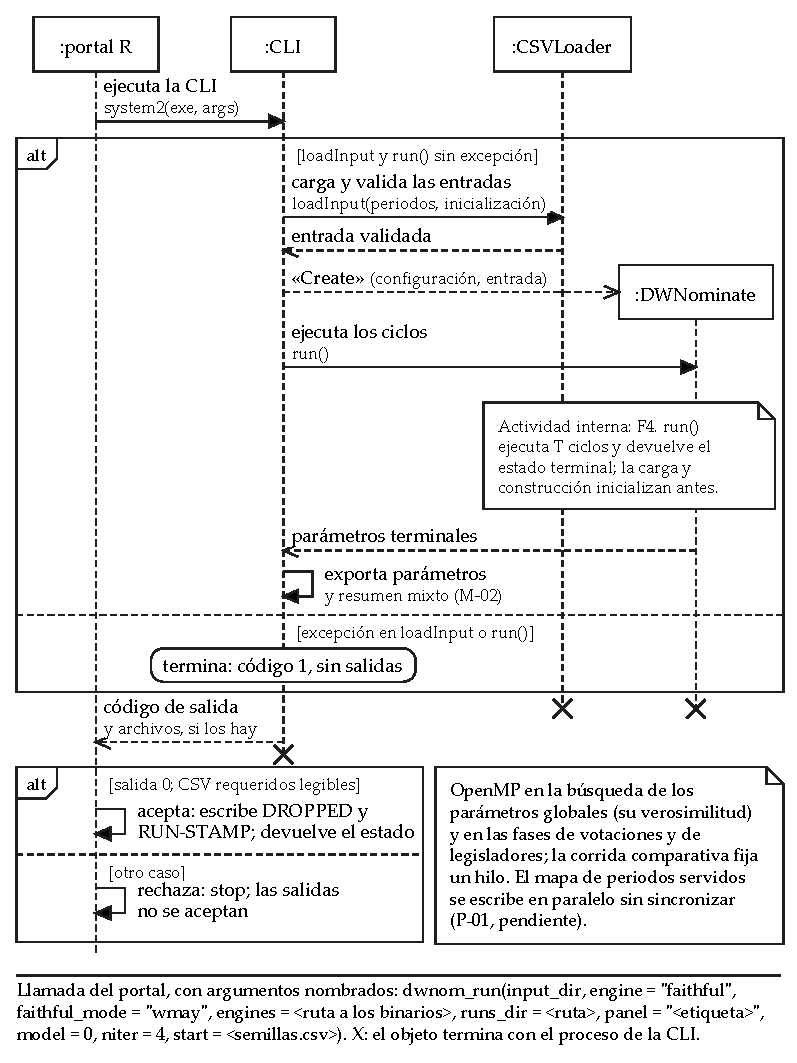
\includegraphics[width=13.5cm]{A2-secuencia-estimacion.pdf}}
\caption[A2. Secuencia de una estimación]{Secuencia de una estimación con el motor fiel desde
el portal en R: salida cero y CSV requeridos legibles, sin validar cobertura completa (D-29).}
\label{fig:A2}
\end{figure}

\chapter[Registro completo de decisiones de diseño][Registro de decisiones]{Registro completo de decisiones de diseño}
\label{anexo:decisiones}

D-01 a D-21 provienen del registro del documento de tesis, fechado en su conjunto al 2 de
octubre de 2026; D-22 a D-32 se agregaron en esta etapa al releer el código para las vistas.
La razón y la evidencia de las decisiones que explican las vistas están en el cuadro
\ref{tab:decisiones}, y la sección \ref{sec:registros} las agrupa en nueve registros.

\footnotesize
\begin{longtable}{L{0.8cm}L{3.5cm}L{2.7cm}L{3.2cm}L{1.85cm}}
\caption[Registro de decisiones de diseño.]{Registro de decisiones de diseño, con la
alternativa descartada, la consecuencia y el estado de cada una.}\label{tab:decisiones-completo}\\
\toprule
Id & Decisión & Alternativa descartada & Consecuencia & Estado \\
\midrule
\endfirsthead
\multicolumn{5}{l}{\footnotesize\emph{Cuadro \ref{tab:decisiones-completo}, continuación}}\\
\toprule
Id & Decisión & Alternativa descartada & Consecuencia & Estado \\
\midrule
\endhead
\bottomrule
\endfoot
D-01 & \texttt{DGESDD} de LAPACK de referencia como rutina predeterminada de
descomposición; sin sustitución silenciosa & descomposición de Eigen con sustitución
automática & la configuración se detiene si falta la biblioteca; cada corrida registra la
rutina & vigente \\
D-02 & perfil sin \texttt{fast-math} ni \texttt{march=native} & aritmética relajada &
comparabilidad entre máquinas por verificar, no identidad demostrada &
vigente \\
D-03 & ninguna reducción de punto flotante dentro de regiones paralelas & reducción de OpenMP
sobre la verosimilitud & suma de parciales en orden de índice; identidad de salidas con
varios hilos pendiente de P-01 e I1 & vigente \\
D-04 & ausentes conservados en la geometría del plano de corte, como en la referencia &
filtrarlos de la nube de puntos & el modo anterior queda disponible por variable de entorno y
se registra & vigente \\
D-05 & valores iniciales canónicos por legislador y periodo, generados con el estimador
estático y versionados con el motor & valores iniciales constantes por legislador & los
valores iniciales son parte del instrumento y se regeneran en cada réplica & vigente \\
D-06 & grado efectivo por legislador según periodos servidos; grado lineal como
especificación principal & grado uniforme por panel; cuadrático como principal & coordenadas:
grado efectivo por trayectoria; resumen: histograma por grado
& vigente \\
D-07 & ciclos externos igualados y truncamiento fijo declarado; ninguna afirmación de
convergencia & regla de parada aplicada a ambos motores & prohíbe un requisito de
convergencia; la comparación solo vale a ciclos iguales & vigente \\
D-08 & cada ejecución registra rutina de descomposición, tratamiento de ausencias y marco de
exportación & declarar la configuración solo en la documentación & un resultado sin sello se
regenera en lugar de citarse & vigente \\
D-09 & proyecciones a la bola unitaria conservadas en los tres sitios de la referencia &
eliminarlas & fidelidad procedimental aunque no cambien el acuerdo & vigente \\
D-10 & exportación en el tiempo normalizado de cada legislador, solo periodos servidos &
rejilla global de periodos & el archivo exportado es la configuración ajustada & vigente \\
D-11 & el fiel conserva sus rutinas; búsquedas NLopt solo en el moderno & adoptar NLopt
en el motor fiel & la pregunta de fidelidad y la de mejora se responden con motores
distintos & vigente \\
D-12 & los motores se comparan y nunca se combinan & elegir un mejor motor & toda fila de
resultado nombra motor, evaluador y rutina de descomposición; las variantes híbridas del
repositorio son experimentales y quedan fuera de todo resultado & vigente \\
D-13 & búsqueda escalar local recentrada en el motor moderno & solución condicional exacta
global & evita el colapso de la segunda dimensión en el primer ciclo & vigente \\
D-14 & tres niveles de verificación con un evaluador común & coincidencia de salidas
finales & un defecto que reproduce la primera dimensión no pasa & vigente \\
D-15 & falsación: la decisión de aceptación rechaza cada versión con un defecto real
reintroducido; para RNF01 se propone situar los umbrales entre un valor defectuoso y uno
corregido & umbrales leídos de una corrida que pasa & la prueba puede fallar; el valor del
umbral corresponde al propietario & vigente; umbral propuesto \\
D-16 & ventana igualada de doce unidades como diseño principal; los demás como sensibilidad
& ventana expansiva como principal & un marco; el bootstrap corre sobre él & propuesta,
pendiente de ratificación \\
D-17 & inferencia solo sobre la primera dimensión; estimación en dos & inferencia en ambas &
la segunda dimensión se describe siempre con su advertencia & vigente \\
D-18 & repositorio público con resultados congelados y licencias; generadores del estudio en
el repositorio de investigación & publicar todo el flujo & la reejecución completa en un
solo comando queda pendiente & vigente \\
D-19 & dos desviaciones declaradas de la referencia: las búsquedas escalares restauran al
salir el mejor estado observado; la restricción de separación que en la referencia es
código inalcanzable no se porta & portar el bucle y la restricción literalmente & fidelidad
procedimental con dos excepciones documentadas en el código y en el registro & vigente \\
D-20 & una mejora de rendimiento fiel exige identidad de salidas numéricas a uno y varios
hilos; metadatos variables se validan aparte & aceptar mejoras dentro de
una tolerancia numérica & la medición antes y después compara solo tiempo; un cambio que
altera un bit es un cambio numérico con su propia verificación & propuesta \\
D-21 & línea base de rendimiento reconstruida antes de cualquier cambio, con repeticiones,
el mismo reloj para todos los brazos y la máquina y la compilación registradas & usar los
tiempos publicados como línea base & los tiempos publicados, de una corrida por celda, no
sirven de línea base & propuesta \\
\addlinespace
D-22 & estado numérico concentrado en \texttt{DWNominate}, trazado miembro a miembro a la
referencia; fases como métodos en el orden original & repartir el estado en objetos por fase
& la estructura no es la que un diseño nuevo elegiría; el motor puede detenerse entre fases &
vigente \\
D-23 & búsquedas como funciones libres con su contexto por argumento & métodos del
orquestador & cada búsqueda puede ejecutarse aislada & vigente \\
D-24 & salvaguarda \texttt{GRID} de 2004 tras un interruptor, apagada en el perfil comparado &
portar un solo linaje & el motor fiel se compara con ambos linajes; el sello registra el modo
& vigente \\
D-25 & perfil de replicación para el brazo medido del motor moderno & medirlo con sus opciones
por omisión & fuera del perfil el moderno cambia más que las búsquedas & vigente \\
D-26 & origen para el legislador sin semilla; la rampa anterior, por variable de entorno &
rampa según la posición en el padrón & arranque neutral, como la referencia; la variable no
reproduce bit a bit el binario anterior & vigente \\
D-27 & el portal rechaza sembrar en proceso un panel de varios periodos & sembrar sobre el
primer periodo & exige una semilla por periodo o un archivo explícito & vigente \\
D-28 & el portal fija el número de hilos y exige uno para Fortran y fiel & dejar los hilos al
entorno & toda comparación a un hilo; el sello registra los hilos & vigente \\
D-29 & salida cero, CSV requeridos legibles y directorio inicialmente vacío;
excluidos como valor de retorno & leer lo que haya en el directorio & rechaza archivos
faltantes o previos; cobertura y esquema completos por verificar & vigente \\
D-30 & sello de cada corrida junto al estado & confiar en la documentación & si el motor no
informa su SVD, el sello la infiere de la construcción y la marca como inferida & vigente \\
D-31 & soporte con \texttt{std::sort} y la descomposición espectral de Eigen & port literal de
\texttt{RSORT} y \texttt{RS} & el orden de los empates puede diferir del de \texttt{RSORT} &
vigente; efecto no medido \\
D-32 & el moderno aborta si la LL previa es finita y $\Delta\ell<-10^{-8}$ & continuar y
exportar & inferencia: detectar una violación del contrato de bloque & vigente \\
\end{longtable}
\normalsize

\chapter[Correspondencia entre las rutinas Fortran y los módulos C++][Correspondencia Fortran y C++]{Correspondencia entre las rutinas Fortran y los módulos C++}
\label{anexo:correspondencia}

Este anexo da el catálogo rutina a rutina que la vista F3 resume (cuadro
\ref{tab:correspondencia}) y las piezas que existen solo en una de las dos variantes Fortran
(cuadro \ref{tab:variantes}).

\begin{table}[H]
\centering
\caption{Módulos del motor fiel y la rutina del programa de referencia que cada uno porta.}
\label{tab:correspondencia}
\footnotesize
\begin{tabular}{L{3.3cm}L{5.8cm}L{3.2cm}}
\toprule
Módulo & Responsabilidad & Rutina de referencia \\
\midrule
\archivo{main_cli} & Línea de comandos, detección de periodos, escritura de salidas y
sellos & programa principal (2004); \texttt{dwnom} y el envoltorio standalone (wmay) \\
\archivo{csv_loader} & Lectura del panel y de los valores iniciales; disposición apilada por
legislador y periodo & lectura de datos \\
\texttt{dwnominate} & Orquestador: estado del modelo y ciclo externo con sus cuatro fases &
\texttt{dwnom} \\
\texttt{likelihood} & Verosimilitud global y estadísticos de clasificación, secuencial y
paralela & \texttt{PLOG} \\
\archivo{normal_cdf} & Tabla precalculada de la distribución normal y sus consultas &
\archivo{init_zdf}, tabla ZDF \\
\archivo{grid_optimizer} & Búsqueda escalar local por pasos para $\beta$ y $w_2$ &
\texttt{SIGMAS}, \texttt{WINT} \\
\archivo{rollcall_derivatives} & Verosimilitud y gradientes por votación & \texttt{PROLLC2} \\
\archivo{rollcall_optimizer} & Búsquedas lineales alternadas de separación y punto medio
& \texttt{RCINT2} \\
\archivo{legislator_derivatives} & Verosimilitud, gradientes e información por legislador
sobre la trayectoria & \texttt{PROX} \\
\archivo{optimize_legislators} & Inicialización por mínimos cuadrados y búsqueda término
a término & \texttt{XINT}; \texttt{GRID} (solo 2004; tras un interruptor, D-24) \\
\archivo{cutting_plane} & Clasificación por plano de corte y dirección de mínima varianza
& \texttt{CUTPLANE}, \texttt{SEARCH} \\
\archivo{cutting_point} & Punto de corte óptimo en una dimensión; códigos de voto;
polaridad & \texttt{JAN1PT}, \texttt{JAN11PT} \\
\archivo{simple_ols}, \archivo{sort_utils} & Pseudoinversa por descomposición espectral de
Eigen con el umbral de la referencia; ordenamiento por índices con \texttt{std::sort}, no un
port del algoritmo de \texttt{RSORT} (D-31) & \texttt{REGA} (con \texttt{RS} en 2004,
\texttt{DSYEV} en wmay), \texttt{RSORT} \\
\bottomrule
\end{tabular}
\end{table}

\begin{table}[H]
\centering
\caption{Piezas propias de cada variante Fortran y su tratamiento en el motor fiel.}
\label{tab:variantes}
\footnotesize
\begin{tabular}{L{2.4cm}L{5.0cm}L{4.9cm}}
\toprule
Variante & Piezas propias & En el motor fiel \\
\midrule
Original 2004 & salvaguarda \texttt{GRID}; descomposición \texttt{LSVRR} de IMSL y su
manejo de errores; \texttt{RS} de EISPACK; formato fijo de entrada; estado en bloques
\texttt{COMMON} (\texttt{/XXCOM/}, \texttt{/MINE/}) & \texttt{GRID} portado tras un
interruptor y apagado en el modo wmay (D-24); \texttt{DGESDD} por omisión (D-01); descomposición
espectral de Eigen (D-31) \\
\addlinespace
wmay & \texttt{DGESDD} y \texttt{DSYEV} de LAPACK; acoplamiento para R; envoltorio
standalone; estado en módulos (\archivo{xxcom_mod}, \archivo{mine_mod}, \archivo{zdf_mod}),
con un \texttt{COMMON /AREA1/} residual en \texttt{REGA}; sin \texttt{GRID} & configuración
igualada en el modo wmay: \texttt{DGESDD}, sin \texttt{GRID}; es la referencia de
reproducción y el evaluador común \\
\bottomrule
\end{tabular}
\end{table}

\section*{Dependencias de módulos C++}

Separadas de F3, las inclusiones verificadas de cabeceras se resumen a un nivel de módulo.
Orquestación incluye directamente los cuatro grupos; se listan también las inclusiones
internas, sin confundirlas con correspondencia histórica ni afirmar ocultamiento completo.

\begin{table}[htbp]
\centering\footnotesize
\caption{Adyacencia de inclusiones entre grupos del motor fiel.}
\begin{tabular}{L{3.0cm}L{4.0cm}L{5.4cm}}
\toprule
Cliente & Proveedor & Evidencia en cabeceras \\
\midrule
Orquestación & búsquedas, geometría, modelo, soporte & \archivo{dwnominate.hpp:14--23} \\
Búsquedas & modelo y soporte & \archivo{grid_optimizer.hpp:12--13}; \archivo{rollcall_optimizer.hpp:12}; \archivo{optimize_legislators.hpp:10--12} \\
Modelo & soporte & \archivo{likelihood.hpp:4} \\
Geometría & soporte & \archivo{cutting_plane.hpp:10}; \archivo{cutting_point.hpp:9} \\
\bottomrule
\end{tabular}
\end{table}

\chapter[Construcción, configuración y manejo de errores][Construcción y errores]{Construcción, configuración y manejo de errores}
\label{anexo:construccion}

Este anexo da la vista física del instrumento \parencite[cap.~2]{swebok2025}: cómo se
construyen los tres binarios y el portal en R, qué configuración fija su resultado (cuadro
\ref{tab:construccion}), y cómo responde cada componente a un error \parencite[cap.~3,
§3.5]{swebok2025} (cuadro \ref{tab:errores}). Las rutas siguen la convención del cuadro
\ref{tab:decisiones}.

\begin{table}[H]
\centering
\caption{Construcción y configuración de los tres binarios y del portal en R.}
\label{tab:construccion}
\footnotesize
\begin{tabular}{L{2.3cm}L{3.0cm}L{3.2cm}L{3.6cm}}
\toprule
Componente & Construcción & Dependencias & Configuración que fija el resultado \\
\midrule
Referencia wmay standalone & gfortran; \archivo{DW-NOMINATE-wmay.f} sin cambios, con
\archivo{r_compat.f90} en lugar de las rutinas de impresión y salida de R y
\archivo{standalone_main.f90} & LAPACK y BLAS al enlazar (\texttt{DGESDD}, \texttt{DSYEV}) &
lee y escribe archivos; solo semilla por legislador; modo \texttt{evaluate}; se ejecuta desde
su directorio, que no crea la salida. El original 2004 se compila aparte y es autocontenido \\
\addlinespace
Motor fiel & C++17 con CMake; \texttt{-O3} sin \emph{fast-math} ni \texttt{-march=native} &
OpenMP y Eigen 3.4.0, obligatorios; LAPACK para \texttt{DGESDD}
(\archivo{USE_SYSTEM_DGESDD}, encendida) & sin LAPACK o sin Eigen la construcción se detiene;
la ruta Eigen solo con la opción apagada, y avisa si cae a Jacobi; el resumen registra la SVD
y el marco de exportación; hilos por \archivo{OMP_NUM_THREADS} \\
\addlinespace
Motor moderno & C++20 con CMake; sin \emph{fast-math} & Eigen y NLopt, descargados si no
están instalados; OpenMP opcional, apagado por omisión; LAPACK para \texttt{DGESDD} & misma
detención si falta LAPACK; pruebas con \texttt{BUILD\_TESTING}; \archivo{--threads}, que el
resumen registra \\
\addlinespace
Portal en R (\archivo{dwnom.R}) & R base & \texttt{wnominate} y \texttt{pscl}, solo para
sembrar en proceso & ubica los binarios según la disposición del repositorio; fija hilos,
perfil y semilla (D-24, D-25, D-28); sella la corrida (D-30) \\
\bottomrule
\end{tabular}
\end{table}

\footnotesize
\begin{longtable}{L{4.0cm}L{1.9cm}L{3.6cm}L{2.8cm}}
\caption{Manejo de errores y excepciones, por componente.}\label{tab:errores}\\
\toprule
Condición & Dónde & Respuesta & Evidencia \\
\midrule
\endfirsthead
\multicolumn{4}{l}{\footnotesize\emph{Cuadro \ref{tab:errores}, continuación}}\\
\toprule
Condición & Dónde & Respuesta & Evidencia \\
\midrule
\endhead
\bottomrule
\endfoot
falta LAPACK con \texttt{DGESDD} encendida, o falta Eigen o NLopt & CMake & error de
configuración; no hay binario & F \archivo{CMakeLists.txt:62}, \archivo{:100}; M
\archivo{CMakeLists.txt:44, 58, 76} \\
falta LAPACKE en la ruta de Eigen & CMake, fiel & aviso explícito; se usa Jacobi y el
resumen lo registra & F \archivo{CMakeLists.txt:84} \\
no hay matrices de votos o no se puede crear el directorio de salida & CLI & mensaje y código
1 & F \archivo{main_cli.cpp:460-485} \\
falta o no se lee una matriz o el archivo de semillas & carga & excepción; código 1, sin
salidas & F \archivo{csv_loader.cpp:130, 292}, \archivo{main_cli.cpp:539-547} \\
excepción durante la ejecución, como una falla de \texttt{DGESDD} & motor & código 1, sin
salidas & F \archivo{cutting_plane.cpp:313, 323}, \archivo{main_cli.cpp:583-586} \\
excepción al construir el motor & CLI, fiel & no se captura: la llamada está fuera de todo
bloque \texttt{try} y el proceso termina de forma anormal & F \archivo{main_cli.cpp:576} \\
no se puede abrir un archivo de salida & salida, fiel & lo omite con un mensaje y
termina con código 0; el portal rechaza la corrida por archivo faltante & F
\archivo{main_cli.cpp:228-231}; R 387-391 \\
argumento desconocido & CLI & aviso; la corrida sigue & F \archivo{main_cli.cpp:175} \\
LL previa finita y $\Delta\ell<-10^{-8}$ entre ciclos & motor moderno & excepción; código 1 & M
\archivo{dwnominate.cpp:388-393} \\
binario inexistente; hilos distintos de uno para Fortran o fiel; margen de la minoría distinto de 0,025;
\texttt{periods} distinto del panel; directorio de salida con archivos & portal & detención
antes de invocar el motor & R 84, 263, 268, 274, 279 \\
sembrar en proceso un panel de varios periodos; semilla por fila para wmay; semilla con
identificadores repetidos o coordenadas no finitas & portal & detención antes de invocar el
motor & R 293-299, 304, 320-326 \\
código de salida distinto de cero; faltan coordenadas, parámetros o resumen & portal &
detención; las salidas no se aceptan & R 380-391 \\
legislador que vota y no queda colocado & portal & no es error: fila en \archivo{DROPPED.csv}
y en el valor de retorno & R 394-416 \\
\end{longtable}
\normalsize

\chapter{Contratos de archivos}
\label{anexo:contratos}

Este anexo fija el contrato de archivos de los motores que la vista F6 abstrae (cuadro
\ref{tab:contratos}) y las reglas de resolución de registros que la figura declara con
multiplicidades opcionales.

\begin{table}[H]
\centering
\caption[Contrato de archivos de los motores.]{Contrato de archivos de los motores. Todas
las salidas van al directorio indicado en la línea de comandos; la referencia escribe un
estado equivalente con otros nombres de archivo y de campo.}
\label{tab:contratos}
\footnotesize
\begin{tabular}{L{3.6cm}L{5.2cm}L{3.6cm}}
\toprule
Archivo & Contenido & Observación \\
\midrule
\multicolumn{3}{l}{\emph{Entradas}} \\
\archivo{votes_matrix_p<N>.csv} & fila por legislador, columna por votación; códigos de la
referencia: 1 a 3 a favor, 4 a 6 en contra, 0 o mayor que 6 ausente; celda vacía o ilegible,
ausente & un archivo por periodo, numerados desde 1 sin huecos; el portal escribe 9 como
ausente \\
\archivo{legislator_metadata.csv} & identificador, nombre, partido, región, distrito &
inerte para la estimación \\
\archivo{wnominate_coordinates.csv} & semilla por legislador: identificador y dos coordenadas &
el binario exige el archivo, no cada legislador; único contrato que wmay admite \\
semilla por fila (\archivo{--seed-per-period}) & identificador, periodo, dos coordenadas &
opcional; prioridad sobre la anterior \\
parámetros de votación de referencia & sesión, identificador, punto medio y separación por
dimensión & opcional; si falta, parten en cero \\
\addlinespace
\multicolumn{3}{l}{\emph{Salidas}} \\
\archivo{cpp_coordinates_all_periods.csv} & legislador, periodo, coordenadas, grado
efectivo & solo periodos servidos; marco del optimizador \\
variante \archivo{_corrected} & las mismas coordenadas con los signos invertidos según la
regla de orientación & no es un nuevo ajuste \\
\archivo{cpp_bill_parameters.csv} & votación, punto medio y separación por dimensión &
índice global de votación \\
\archivo{cpp_summary.csv} & verosimilitud, ciclos, votos válidos, clasificación, pesos,
grado pedido, histograma de grado efectivo y tiempo & LL terminal; clasificación de fase
previa (M-02); SVD, ausencias y marco registrados \\
\archivo{RUN-STAMP.csv}, \archivo{DROPPED.csv} & sello de la corrida y excluidos, escritos por
el portal & junto al estado; el portal también los devuelve \\
\bottomrule
\end{tabular}
\end{table}

Reglas de resolución. El padrón y los archivos de semillas son registros crudos: pueden traer
identificadores fuera del panel, y el motor no exige que cada registro calce con exactamente
una fila servida; el portal sí rechaza una semilla con identificadores repetidos. El
emparejamiento de coordenadas entre corridas es por (legislador, periodo), sin validación uno
a uno. La identidad del panel requiere hashes de las matrices, del orden de identificadores
de legisladores, votaciones y periodos, de los archivos de semillas y de la configuración.
Se conserva la procedencia en los manifiestos de linaje y en \archivo{RUN-STAMP.csv}
(binario, semilla, argumentos y backend), sin atribuir al sello hashes que no escribe.
Los recuentos crudos, no ausentes y ajustados son diagnósticos separados; no identifican la matriz.

\chapter{Perfil de ejecución}
\label{anexo:perfil}

Este anexo reúne en el cuadro de perfil de ejecución (cuadro \ref{tab:perfil}) las banderas,
la rutina de SVD, los hilos, el arranque, el evaluador de la verosimilitud, los ciclos y el
contrato de semillas que las vistas F4, T5 y F7 dejan fuera de las cajas, junto con las
invocaciones del protocolo de reproducción wmay. Este cuadro fija esa comparación de tres
brazos; el protocolo original 2004 (cuadro \ref{tab:protocolos}) declara sus diferencias.
El bootstrap regenera semillas por periodo y elegibilidad por réplica (algoritmo \ref{alg:bootstrap}).

\footnotesize
\begin{longtable}{L{2.6cm}L{5.0cm}L{4.8cm}}
\caption[Perfil de ejecución.]{Perfil de ejecución de los motores, con el perfil
comparado.}\label{tab:perfil}\\
\toprule
Aspecto & Opción, variable o invocación & Perfil comparado y observación \\
\midrule
\endfirsthead
\multicolumn{3}{l}{\footnotesize\emph{Cuadro \ref{tab:perfil}, continuación}}\\
\toprule
Aspecto & Opción, variable o invocación & Perfil comparado y observación \\
\midrule
\endhead
\bottomrule
\endfoot
Entradas y salidas & \archivo{--input-dir}, \archivo{--output-dir}, \archivo{--wnominate},
\archivo{--seed-per-period} & código de salida distinto de cero si falta una matriz o el
archivo de semillas (cuadro \ref{tab:errores}) \\
\addlinespace
Estimación & \archivo{--model} (grado), \archivo{--iterations} (ciclos), \archivo{--periods},
\archivo{--dimensions} & grado declarado por panel; cuatro ciclos; dos dimensiones; en una
dimensión no se ajusta el peso y el corte usa \texttt{JAN11PT} \\
\addlinespace
Contrato de semillas & semilla por legislador o por fila & por legislador en todos los
brazos, único contrato que wmay admite; por fila solo como control \\
\addlinespace
Linaje del motor fiel & \archivo{--wmay-replication}; en el portal, el modo wmay o el de la
salvaguarda de 2004 & modo wmay: \texttt{GRID} apagado (D-24) \\
\addlinespace
Perfil del motor moderno & \archivo{--fortran-replication}; el portal añade
\archivo{--optimizer-precision=strict} & fija las opciones canónicas (COBYLA, búsqueda escalar
local, votaciones desde cero, sin identificación adicional ni tolerancias adaptativas, iguales
a las de omisión); cambia la tabla de verosimilitud, la de la referencia en lugar de la normal
continua, y retira las cotas globales de $w_2$ y $\beta$ (D-25) \\
\addlinespace
Búsquedas del motor moderno & \archivo{--scalar-search}, \archivo{--block-solver} & local y
COBYLA en el perfil comparado \\
\addlinespace
Parada opcional del moderno & \archivo{--convergence-abs}, \archivo{--convergence-rel},
\archivo{--convergence-patience}, \archivo{--min-iterations} & desactivada por omisión
(tolerancias en cero); nunca criterio de parada en una comparación (D-07) \\
\addlinespace
Arranque & escalares iniciales de la referencia; votaciones en cero; legislador sin semilla
en el origen & iguales en ambos motores (D-25, D-26) \\
\addlinespace
Evaluador de la verosimilitud & fiel: tabla precalculada de la referencia; moderno:
\archivo{--likelihood} (continua por omisión) & tabla de la referencia en ambos motores (D-25)
\\
\addlinespace
Rutina de SVD & \archivo{USE_SYSTEM_DGESDD} (fiel), \archivo{DWNOMINATE_USE_SYSTEM_DGESDD}
(moderno) & \texttt{DGESDD}; registrada en el resumen del fiel y en el sello (D-01, D-30) \\
\addlinespace
Hilos & \archivo{OMP_NUM_THREADS} (fiel); \archivo{--threads} (moderno) & uno en toda
comparación, impuesto por el portal (D-28) \\
\addlinespace
Modos anteriores del fiel & \archivo{DWNOM_EXPORT_GLOBAL_T},
\archivo{DWNOM_CUTPLANE_FILTER_ABSENT}, \archivo{DWNOM_SEED_FALLBACK_RAMP} & conservan
comportamientos previos a una corrección; los que cambian un número publicado quedan en el
resumen \\
\addlinespace
Volcado de fases & \archivo{DWNOM_PHASE_DUMP} & registro por votación con marcas de fase para
el nivel de componente; inerte en otro caso \\
\addlinespace
Llamada desde el portal & \texttt{dwnom\_run} con directorio de entrada, motor, binarios,
directorio de corridas, panel, grado, ciclos y semillas & devuelve coordenadas, parámetros,
escalares, excluidos y sello; salida cero y CSV requeridos legibles (figura
\ref{fig:A2}) \\
\addlinespace
Reevaluación bajo evaluador común & \archivo{stage_terminal_state.py}; wmay standalone en modo
\texttt{evaluate} & cero ciclos; el arnés exige su directorio de trabajo \\
\addlinespace
Comparación de coordenadas & \archivo{map_agreement.py} & emparejamiento por (legislador,
periodo); alineación ortogonal sin reescalar; marco global o por periodo declarado \\
\end{longtable}
\normalsize

\chapter{Narrativas de los casos de uso}
\label{anexo:narrativas}

Este anexo da, para cada caso de uso de la vista F2, la precondición, la condición de fallo y
el criterio de término que la figura no dibuja (cuadro \ref{tab:narrativas}).

\footnotesize
\begin{longtable}{L{2.6cm}L{3.2cm}L{3.2cm}L{3.2cm}}
\caption{Narrativas de los casos de uso: precondición, fallo y término.}\label{tab:narrativas}\\
\toprule
Caso de uso & Precondición & Fallo & Término \\
\midrule
\endfirsthead
\multicolumn{4}{l}{\footnotesize\emph{Cuadro \ref{tab:narrativas}, continuación}}\\
\toprule
Caso de uso & Precondición & Fallo & Término \\
\midrule
\endhead
\bottomrule
\endfoot
Declarar panel y semillas (RF01, RF02) & directorio de panel con una matriz por periodo y el
archivo de semillas por legislador; opcionalmente semillas por fila y parámetros de votación
de referencia & falta una matriz o el archivo de semillas: error y código de salida distinto
de cero, sin salidas & el motor reporta cuántas coordenadas iniciales aplicó por cada vía,
cuántos legisladores partieron del origen o quedaron excluidos y qué grado efectivo recibió
cada uno; un argumento desconocido y la ausencia del archivo opcional se aceptan con aviso \\
\addlinespace
Estimar estático o dinámico (RF03, RF04) & entradas declaradas; perfil de la corrida
(dimensiones, grado, ciclos) & código de salida distinto de cero, o salida cero con archivos
incompletos: el portal rechaza la corrida & directorio de estado con coordenadas, parámetros
de votación y resumen con su procedencia; código de salida cero \\
\addlinespace
Validar con el caso chileno (RF10 a RF12) & ajuste observado sobre el panel del 55.º
periodo; cortes y cohortes fijados desde el calendario antes de inspeccionar estimación
alguna & una réplica cuyo número de periodos difiera del observado o cuyo grado efectivo
exceda el lineal se rechaza; la orientación de la primera dimensión se verifica antes de
leer réplica alguna & por (cohorte, partido): desplazamiento, cotas, valor $p$ ajustado e
indicador de robustez, con rejilla, grado, valores iniciales y motor declarados \\
\addlinespace
Verificar y comparar (RF08, RF09) & dos corridas controladas que superan el control de
paridad de entradas: mismo panel, semillas, ciclos, grado, códigos y margen de la minoría, marco de
exportación y configuración de compilación & una cláusula de paridad que falla: la
comparación no se ejecuta; una discrepancia con sello distinto se reporta como configuración
distinta, no como defecto & informe de comparación: diferencia de verosimilitud bajo
evaluador común, desacuerdo absoluto por votación, correlaciones por dimensión, razón de
amplitud, peso de la segunda dimensión de ambos motores y reflexiones, con cobertura y marco
declarados \\
\end{longtable}
\normalsize

\chapter[Conjunto de paneles de prueba y ajustes igualados][Paneles de prueba]{Conjunto de paneles de prueba y ajustes igualados}
\label{anexo:paneles}

Este anexo detalla el conjunto de paneles de las pruebas exhaustivas (cuadro
\ref{tab:paneles}) y los estadísticos y ajustes igualados que la sección
\ref{sec:experimental} resume (cuadro \ref{tab:estadisticos}).

\begin{table}[H]
\centering
\caption[Conjunto de paneles de prueba.]{Conjunto de paneles de prueba. La descripción identifica el escenario; los hashes de
matriz, orden, semillas y configuración identifican la entrada. Los recuentos son diagnósticos.}
\label{tab:paneles}
\footnotesize
\begin{tabular}{L{3.4cm}L{3.9cm}L{1.5cm}L{3.5cm}}
\toprule
Panel & Escenario & Grado & Brazos de referencia \\
\midrule
Legislaturas 353, 366 y 368 (estáticos) & una legislatura cada uno; bytes idénticos a un
periodo del panel de 23 periodos de la curación anterior & 0 & referencia, fiel, moderno \\
Senado de EE.\,UU., 90.º Congreso (estático) & un periodo; comparación externa & 0 &
referencia, fiel, moderno \\
Senado de EE.\,UU., Congresos 111 a 115 & cinco periodos; valores iniciales reparados & 1 &
los tres, en dos máquinas \\
Cámara de Diputados 2002--2022 & 23 periodos, extendido a marzo de 2022 & 1 & los tres, en
dos máquinas \\
Cámara de Diputados, curación anterior & 23 periodos, legislaturas 346 a 368 & 2 & los tres \\
55.º periodo legislativo & doce unidades de cuatro meses & 1 & referencia; el brazo fiel
debe congelarse \\
Sintéticos (tres niveles de información en la segunda dimensión) & verdad conocida por
construcción & 0 & archivos de verdad \\
\bottomrule
\end{tabular}
\end{table}

\footnotesize
\begin{longtable}{L{3.5cm}L{8.9cm}}
\caption[Estadísticos y ajustes igualados de las pruebas exhaustivas.]{Estadísticos de las
pruebas exhaustivas, por nivel de verificación, y ajustes del protocolo wmay de tres brazos.
La aceptación contra 2004 registra las diferencias del cuadro \ref{tab:protocolos}; RNF01 queda abierto.}\label{tab:estadisticos}\\
\toprule
Elemento & Especificación \\
\midrule
\endfirsthead
\multicolumn{2}{l}{\footnotesize\emph{Cuadro \ref{tab:estadisticos}, continuación}}\\
\toprule
Elemento & Especificación \\
\midrule
\endhead
\bottomrule
\endfoot
\multicolumn{2}{l}{\emph{Estadísticos, por nivel}} \\
Componente & tasa de error del plano de corte; identidad de los escalares tras el primer
ciclo \\
Estado & diferencia de verosimilitud por voto bajo el evaluador común, con el desacuerdo
absoluto por votación al lado; identidad del recuento de votos válidos \\
Mapa & correlaciones por dimensión en el marco global, razón de amplitud, distancia media y
reflexiones \\
Determinismo & identidad de salidas numéricas con uno, dos, cuatro y doce hilos; metadatos aparte \\
\addlinespace
\multicolumn{2}{l}{\emph{Ajustes igualados}} \\
Ciclos & cuatro, la convención de la comparación publicada, declarados en cada sello \\
Grado & el declarado por panel \\
Valores iniciales & en la comparación wmay, por legislador en todos los brazos, porque wmay solo lee esa
forma; los valores por periodo como control \\
Hilos & uno en toda comparación \\
Motor moderno & modo de replicación y precisión estricta \\
Rutina de descomposición & protocolo wmay: \texttt{DGESDD}; original 2004: \texttt{LSVRR}; fiel: backend registrado \\
Aritmética & estricta, sin \emph{fast-math} \\
Escalares iniciales & los de la referencia \\
Dimensiones & dos \\
\end{longtable}
\normalsize

\chapter{Diseño del estudio chileno}
\label{anexo:chile}

Este anexo da el diseño del estudio chileno que la sección \ref{sec:algoritmos} resume: el
contraste, la inferencia y la periodización con su regla de discretización (tarea E3).

El estudio estima el desplazamiento de las medianas de partido en la primera dimensión durante
el 55.º periodo legislativo, dividido en tres fases por el estallido social del 18 de octubre
de 2019, el plebiscito del 25 de octubre de 2020 y el fin del periodo el 10 de marzo de 2022,
cortes fijados desde el calendario antes de inspeccionar estimación alguna. Para el partido
$p$, el contraste es $\Delta_p = m_{p3} - m_{p1}$, con $m_{pk}$ la mediana de la primera
dimensión de sus diputados activos al fin de la fase $k$, y la hipótesis alternativa
unilateral $\Delta_p < 0$ se fijó antes del análisis \parencite{nieves2026jcc}. La inferencia
sigue el bootstrap paramétrico establecido para este estimador
\parencite{lewis2004measuring,carroll2009measuring}: redibujar cada voto desde su probabilidad
ajustada y reestimar todo el instrumento en cada réplica (algoritmo \ref{alg:bootstrap}). Tres
decisiones lo distinguen del uso habitual: los valores iniciales se regeneran dentro de cada
réplica, porque reutilizar los observados con pocos ciclos puede anclar las soluciones; solo
se redibujan las votaciones válidas; y cada réplica se alinea a la primera dimensión observada
por signo y localización (D-17). Un partido se declara robustamente desplazado solo si ambas
cotas son negativas y el valor $p$ ajustado por \textcite{holm1979simple} es menor que el
nivel (RF11).

La subdivisión del tiempo es una elección del analista que los datos no fijan y que mueve el
resultado (RF12); el diseño la trata como un parámetro declarado (cuadro \ref{tab:disenos}).
El principal, propuesto y pendiente de ratificación (D-16), es la ventana igualada: un solo
ajuste sobre las doce unidades de cuatro meses del periodo, en un solo marco, sobre el cual
corre el bootstrap; los otros tres son análisis de sensibilidad. La regla de discretización
tiene tres cláusulas. El grado es siempre lineal, para que una rejilla más fina no cambie la
mezcla de grados efectivos. La unidad debe ser lo bastante corta para que la cohorte que entró
al inicio alcance cinco unidades servidas, el mínimo del término lineal (D-06), y lo bastante
larga para que ninguna unidad quede vacía en el receso de verano: con el umbral de veinte
votos, la de cuatro meses es la más corta que el registro sostiene. Y toda cifra declara
rejilla, grado y valores iniciales. El modelo se estima en dos dimensiones, pero la
inferencia se hace solo sobre la primera (D-17), porque la segunda es considerablemente más
sensible entre implementaciones, optimizadores, horizontes y réplicas
\parencite{nieves2026jcc}.

\begin{table}[H]
\centering
\caption{Diseños de periodización: qué varía cada uno, cómo trata los marcos y qué pregunta
responde.}
\label{tab:disenos}
\footnotesize
\begin{tabular}{L{2.9cm}L{3.5cm}L{2.8cm}L{3.1cm}}
\toprule
Diseño & Varía o fija & Marcos & Pregunta \\
\midrule
Ventana igualada (principal, pendiente de ratificación) & un ajuste; doce unidades de cuatro
meses; grado lineal & un marco; solo el control de orientación & cuánto se desplazaron las
medianas en un marco común \\
\addlinespace
Ventana expansiva & tres ajustes anidados que terminan en cada frontera & rotación estimada en
las unidades de calentamiento & cuánto depende una posición terminal del registro anterior \\
\addlinespace
Por tramos & tres ajustes independientes, uno por fase, con seis unidades internas cada uno &
tres marcos lado a lado & si hubo un salto en la frontera \\
\addlinespace
Ajuste único rebanado & un ajuste sobre las unidades del diseño por tramos & sin realineación
& control de los dos anteriores \\
\bottomrule
\end{tabular}
\end{table}

\chapter[Mejora de rendimiento: cambios candidatos y protocolo][Mejora de rendimiento]{Mejora de rendimiento: cambios candidatos y protocolo}
\label{anexo:rendimiento}

Este anexo da el catálogo completo de cambios candidatos de la mejora de rendimiento del
motor fiel (cuadro \ref{tab:candidatos}) y el protocolo de medición paso a paso (cuadro
\ref{tab:protocolo}) que la sección \ref{sec:rendimiento} resume. Ningún cambio está
implementado. La inserción concurrente P-01 está en la fase de legisladores: el lazo paralelo
inserta en el contenedor de periodos servidos por legislador sin sección crítica, mientras los
coeficientes temporales tienen una preinicialización en serie hecha precisamente para evitar
ese riesgo (F \archivo{dwnominate.cpp:1463-1465}, \archivo{:1478}, \archivo{:1814}); la corrección
es extender esa preinicialización. Por inspección, la carrera no toca los números ajustados,
pero alimenta el marco de exportación.

\footnotesize
\begin{longtable}{L{0.8cm}L{5.3cm}L{2.2cm}L{4.0cm}}
\caption[Cambios candidatos de rendimiento.]{Cambios candidatos de la mejora de rendimiento
del motor fiel, la fase que afectan y su efecto esperado sobre los resultados. Ninguno está
implementado; el efecto esperado es una hipótesis que la condición de aceptación somete a
prueba.}\label{tab:candidatos}\\
\toprule
Id & Cambio & Fase & Efecto esperado en los resultados \\
\midrule
\endfirsthead
\multicolumn{4}{l}{\footnotesize\emph{Cuadro \ref{tab:candidatos}, continuación}}\\
\toprule
Id & Cambio & Fase & Efecto esperado en los resultados \\
\midrule
\endhead
\bottomrule
\endfoot
M-01 & restringir los lazos de cada votación y las evaluaciones globales al bloque de filas
de su periodo & votaciones; verosimilitud global & ninguno: mismas celdas no ausentes, en el
mismo orden \\
M-02 & guardar los votos por bloques de periodo con índice local, contiguos por votación, con
una vista por legislador para los lazos que la usan & todas; carga & ninguno si cada lazo
conserva su orden; reordenar lazos está excluido \\
M-03 & listas precalculadas, en orden ascendente, de los votantes de cada votación y de las
votaciones de cada legislador & votaciones; verosimilitud global & ninguno: mismo orden de
suma \\
M-04 & eliminar asignaciones y copias dentro de los lazos internos; memoria reutilizable por
hilo & todas & ninguno: mismos valores \\
M-05 & evaluar solo la verosimilitud en los puntos de búsqueda lineal y en la primera y
última evaluación de cada votación & votaciones; legisladores & ninguno esperado; se verifica
porque la primera evaluación inicia la historia de la búsqueda \\
M-06 & una sola consulta a la tabla normal por voto para el valor y su logaritmo &
votaciones; verosimilitud & ninguno: mismas entradas de la tabla \\
M-07 & preparar una sola vez los datos invariantes de cada votación y suprimir el trabajo
muerto del plano de corte & votaciones & ninguno: mismos arreglos, en el mismo orden \\
M-08 & guardar invariantes dentro de las búsquedas escalares & escalares & ninguno si se
respeta el orden de evaluación; valor esperado bajo \\
M-09 & carga en tiempo proporcional a los votos válidos & carga & ninguno \\
\addlinespace
X-01 & omitir el plano de corte cuando su resultado se descarta & votaciones & estado
ajustado sin cambio, pero altera el flujo del procedimiento: fuera del alcance sin decisión
del propietario \\
\addlinespace
P-01 & eliminar la inserción concurrente en un contenedor compartido de la fase de
legisladores & legisladores & requisito previo de corrección; no altera los números
ajustados \\
P-02 & registrar el número de hilos en el resumen de cada corrida & salida & requisito
previo de medición; la línea nueva se excluye de la comparación de archivos \\
\end{longtable}
\normalsize

\footnotesize
\begin{longtable}{L{2.2cm}L{6.2cm}L{4.0cm}}
\caption[Protocolo de medición de rendimiento.]{Protocolo de medición de la mejora de
rendimiento: qué fija cada paso y por qué.}\label{tab:protocolo}\\
\toprule
Paso & Qué se fija o se hace & Por qué \\
\midrule
\endfirsthead
\multicolumn{3}{l}{\footnotesize\emph{Cuadro \ref{tab:protocolo}, continuación}}\\
\toprule
Paso & Qué se fija o se hace & Por qué \\
\midrule
\endhead
\bottomrule
\endfoot
Requisitos previos & corregir la inserción concurrente (P-01) y registrar el número de hilos
(P-02) & un resultado no reproducible no puede medirse \\
\addlinespace
Línea base & etiquetar la versión de partida; mismo compilador, opciones, bibliotecas y máquina
para ambas versiones; registrar procesador, memoria, sistema operativo y opciones & los tiempos
publicados no fijan estas condiciones \\
\addlinespace
Paneles & cuatro estáticos y tres dinámicos del cuadro \ref{tab:paneles}; mismos valores
iniciales; cuatro ciclos; dos dimensiones & el tiempo depende del camino de búsqueda \\
\addlinespace
Condición de aceptación & cinco corridas por versión e hilos: parámetros, claves y estadísticas
idénticos; excluir solo tiempo, hilos y fecha; validar esos metadatos aparte & un cambio que
altera un bit es un cambio numérico (D-20) \\
\addlinespace
Perfilado & atribuir el tiempo de la línea base a cada rutina; contadores de acceso a memoria &
elegir cambios por evidencia y contrastar la hipótesis del recorrido \\
\addlinespace
Medición & una corrida de calentamiento descartada; al menos cinco corridas por panel, versión
y número de hilos, intercaladas; mediana, mínimo, máximo y rango intercuartílico; cambio como
cociente de medianas & separar la mejora de la variación de la máquina; comparación principal
a un hilo (RNF04) \\
\addlinespace
Orden y registro & cambios de a uno, primero los de mayor efecto esperado en la fase de
votaciones; resultados en un directorio fechado e inmutable con sus programas generadores & que
un fallo sea atribuible; trazabilidad numérica (RNF06) \\
\end{longtable}
\normalsize

\chapter{Procedencia y evidencia de esta revisión}
\label{anexo:procedencia}

Se verificaron localmente los motores en \archivo{ad945a91} y la investigación en
\archivo{3cb203e3}. Los números de línea del portal R corresponden a su archivo local modificado, SHA-256\par
{\footnotesize\texttt{170d8a4638b312e6a5d83f45d1f0ea417b843d5d50d5a6ab0fd516a767dc0090}}\par
no al blob publicado de la revisión base. La fuente original seleccionada es \archivo{DW-NOMINATE-2004.FOR};
su SHA-256 es\par
{\footnotesize\texttt{276e3cb545f2ba18d4ce4ca193f45ae8695c7e0b343f3dbcb7caaeaaa13d63a8}}\par
El ejecutable original recompilado el 6 de octubre tiene SHA-256\par
{\footnotesize\texttt{08dc4e042e46b67268a0e533ef64ba6a6643a33d6de22b6bda1d6ad13701c2ab}}\par
Los comandos, compilador GNU Fortran 15.2.0, dependencias y hashes completos están en
\href{run:../evidence/lineage/builds/README.md}{la procedencia de builds incluida}.
Esa construcción original usó los flags legacy registrados y wmay usó \texttt{-O2};
sus tiempos no se usan como benchmark. El benchmark E3 exige nuevas condiciones comparables.

Las tres comparaciones dinámicas retenidas original/wmay y sus limitaciones se documentan en
\href{run:../evidence/ENGINE-CLOSEOUT.md}{el registro de linaje incluido}. El motor fiel con
GRID activo no reemplaza esa identificación del original. El paquete conserva fuentes de
código verificadas y manifiestos; no contiene un nuevo replay numérico ni modifica el artículo.

El 8 de octubre la API confirmó la rama pública del motor en \archivo{00ba24c0}, con seis
commits locales de reorganización aún ausentes del remoto; el commit \archivo{ad945a91} no
se pudo recuperar allí. El backlog base y el portal R publicado sí existen en la revisión privada citada
de investigación, pero las propuestas I y la ampliación local del portal no están en esos blobs.
El archivo local del portal coincide con el hash usado en la revisión de figuras del 7 de octubre;
sus números de línea siguen vigentes para esa copia. Se incluye y cita esa fuente local exacta. Esto verifica destinos para la cuenta consultada, no permisos de cada lector.
La evidencia de diseño de esta revisión se entrega en este PDF y en su paquete local.

La planilla de seguimiento pudo leerse mediante el conector: G2 aún figuraba ``Sin empezar'',
con fecha de E2 del 2 de octubre; E3 y H8 no aparecían entre esas filas. El registro de este
informe documenta los artefactos actuales; sincronizar los estados y la fecha de la planilla
con el responsable sigue pendiente. El backlog incluido también conserva G2/E3 sin empezar y H8
pendiente; este informe distingue diseño escrito de aprobación. La API del 8 de octubre devuelve
\texttt{permission=none} y \texttt{pull=false} para Julio (\texttt{jcredberry}) en
\texttt{quevotan-db}; la ruta remota \texttt{tesis/} aún no existe. Publicación y acceso siguen abiertos.
La confirmación del objetivo chileno, RNF01 y la periodización siguen siendo decisiones del
profesor guía. El resultado de esta pasada es un candidato de revisión, no una entrega registrada.


\section*{Propuestas I1--I7 para la Etapa 3}

La revisión final de diseño produjo dieciocho mejoras agrupadas en siete propuestas locales
del backlog. El registro leído las marca \emph{Pendiente}, hasta que Roberto y Pablo las
adopten. No se presentan como implementación realizada ni como tareas E2 incumplidas.

\begin{table}[htbp]
\centering\footnotesize
\caption{Propuestas de la Etapa 3 incorporadas al registro local el 8 de octubre.}
\begin{tabular}{L{0.7cm}L{7.9cm}L{2.0cm}L{1.0cm}}
\toprule
ID & Alcance y relación con este diseño & Responsable & Horas \\
\midrule
I1 & corregir P-01 y verificar salidas idénticas con 1/2/4/12 hilos; prerrequisito de I6 & Pablo & 8 \\
I2 & resumen del estado final, exportación 1D y hilos en resumen & Pablo & 8 \\
I3 & errores y contratos de entrada/salida & Pablo & 8 \\
I4 & modos de prueba por componente accesibles desde la CLI fiel & Pablo & 6 \\
I5 & productor RF09 único, emparejamiento uno a uno & Roberto & 10 \\
I6 & rendimiento a un núcleo y salidas idénticas; original 2004 como referente de tesis,
wmay como antecedente adicional & ambos & 40 \\
I7 & comentarios obsoletos; rutas y dependencia requieren pruebas de ejecución y construcción & Roberto & 3 \\
\bottomrule
\end{tabular}
\end{table}

Las horas son estimaciones propuestas. La copia del backlog local incluida conserva el texto
original de I6 (``contra wmay''); el \href{run:../evidence/ETAPA-3-consistency-proposal-2026-10-08.md}{registro E3 corregido}
alinea la propuesta con el original 2004.
El registro corregido no adopta las tareas ni cambia los responsables. Las pruebas de I1 muestran
el defecto antes y exigen determinismo después; I2 corrige estadísticas antes de congelar I6.

La \href{run:../evidence/performance-candidates-confirmed-2026-10-08.md}{comprobación estática
de candidatos del 8 de octubre} confirma premisas de C1 a C15 y propone N1 a N7; no construye,
ejecuta ni mide mejoras. Precisa que C2 puede trasladar costo a legisladores y verosimilitud,
C6 consume menos resultados de lo supuesto, y C5/C8 tienen un alcance de asignaciones más
estrecho. Son insumos de I6, no resultados del informe.

Antes de optimizar, I1 debe preinicializar el mapa de periodos servidos y endurecer el acceso
al mapa de coeficientes de la misma región paralela; I2 corrige resumen, exportación y sello. Sigue una
línea base reconstruida y perfilada, preservando D-03 y verificando identidad de salidas tras
cada cambio. N1 exige reutilizar solo entradas iguales bit a bit; C14 y N4 omiten evaluaciones
del flujo heredado y requieren una decisión explícita. Los tiempos históricos citados por esa
nota deben regenerarse; no se transfieren como mediciones actuales. El catálogo del anexo
\ref{anexo:rendimiento} conserva el diseño E2 y esta fuente amplía la planificación E3.

La auditoría completa de concurrencia del motor moderno queda como tarea H4 pendiente: revisar
escrituras compartidas y repetir paneles estáticos/dinámicos a 1/2/4/12 hilos con builds e inputs
identificados. P-01 y P-02 se encontraron en el fiel; sus diferencias con el moderno no prueban
seguridad global. No se ejecutó esa auditoría ni un nuevo experimento en esta revisión.


\end{document}
